\documentclass[12pt,a4paper]{article}
\usepackage[a4paper, left=3.5cm, right=2cm, top=2.5cm, bottom=3cm,footskip=.25in]{geometry}
\usepackage[utf8]{inputenc}
\usepackage[T1]{fontenc}
\usepackage{amsmath}
\usepackage{amssymb}
\usepackage{lmodern}
\usepackage{indentfirst}
\usepackage{enumerate}
\usepackage{array}
\usepackage{float}
\usepackage{ragged2e}
\usepackage{lipsum}

\usepackage[pdftex]{graphicx}
\graphicspath{{.png}{images/}}
\renewcommand{\baselinestretch}{1.8}

\usepackage{algorithm}
\usepackage{algpseudocode}
\usepackage{setspace}
\usepackage[table]{xcolor}
\usepackage{booktabs}

\usepackage{pdfpages}

\usepackage{hyperref}
\hypersetup{colorlinks=true, citecolor=violet, linkcolor=black}

\usepackage{titlesec}

\titlespacing*{\section}
{0pt}{6.5ex plus 1ex minus .2ex}{5.3ex plus .2ex}
\titlespacing*{\subsection}
{0pt}{6.5ex plus 1ex minus .2ex}{5.3ex plus .2ex}

\usepackage{etoolbox}

\makeatletter
\patchcmd{\ttlh@hang}{\parindent\z@}{\parindent\z@\leavevmode}{}{}
\patchcmd{\ttlh@hang}{\noindent}{}{}{}
\makeatother

\usepackage{soul}
\newcommand{\ol}[1]{{\setul{-1.2em}{}\ul{#1}}}
\newcommand{\textoverline}[1]{{\setul{-5em}{}$\overline{\mbox{#1}}$}}

\newtheorem{definition}{Definition}[subsection]
\newtheorem{example}{Example}[subsection]

\usepackage[round]{natbib}
\usepackage{tikz-qtree}
\usepackage{tikz}
\usetikzlibrary{arrows}
\usetikzlibrary{decorations.text}

\usepackage{pifont}
\newcommand{\xmark}{\ding{53}}

\begin{document}

\begin{titlepage}
	\centering
	\par\vspace{1cm}
	{\scshape\bf FACULTY OF MATHEMATICS, PHYSICS AND INFORMATICS \par}
	{\scshape\bf COMENIUS UNIVERSITY IN BRATISLAVA \par}
	\par\vspace{8cm}
	{\scshape\bf OPTIMIZATION OF AN ABDUCTIVE REASONER FOR DESCRIPTION LOGICS \par}
	\par\vspace{0.5cm}
	{\textsc Master Thesis \par}
	\par\vspace{10.6cm}
	{\scshape\bf 2019 \hfill Bc. Katarína Fabianová \par}
\end{titlepage}

\pagebreak
\thispagestyle{empty}
\centering
\par\vspace{1cm}
{\scshape\bf FACULTY OF MATHEMATICS, PHYSICS AND INFORMATICS \par}
{\scshape\bf COMENIUS UNIVERSITY IN BRATISLAVA \par}
\par\vspace{8cm}
{\scshape\bf OPTIMIZATION OF AN ABDUCTIVE REASONER FOR DESCRIPTION LOGICS \par}
\par\vspace{0.5cm}
{\textsc Master Thesis \par}
\par\vspace{2cm}
\begin{table*}[ht]
	\newcolumntype{x}[1]{>{\hspace{0pt}}p{#1}}
	\begin{tabular}{@{}x{5cm}x{10cm}@{}}
		Study Program: & Applied Informatics \\
		Field of Study: & 2511 Applied Informatics \\
		School Department: & Department of Applied Informatics \\
		Adviser: & Mgr. Júlia Pukancová, PhD. \\
		Consultant: & RNDr. Martin Homola, PhD. \\
	\end{tabular}
\end{table*}
\par\vspace{5.07cm}
{\scshape\bf Bratislava 2019 \hfill Bc. Katarína Fabianová \par}

\pagebreak

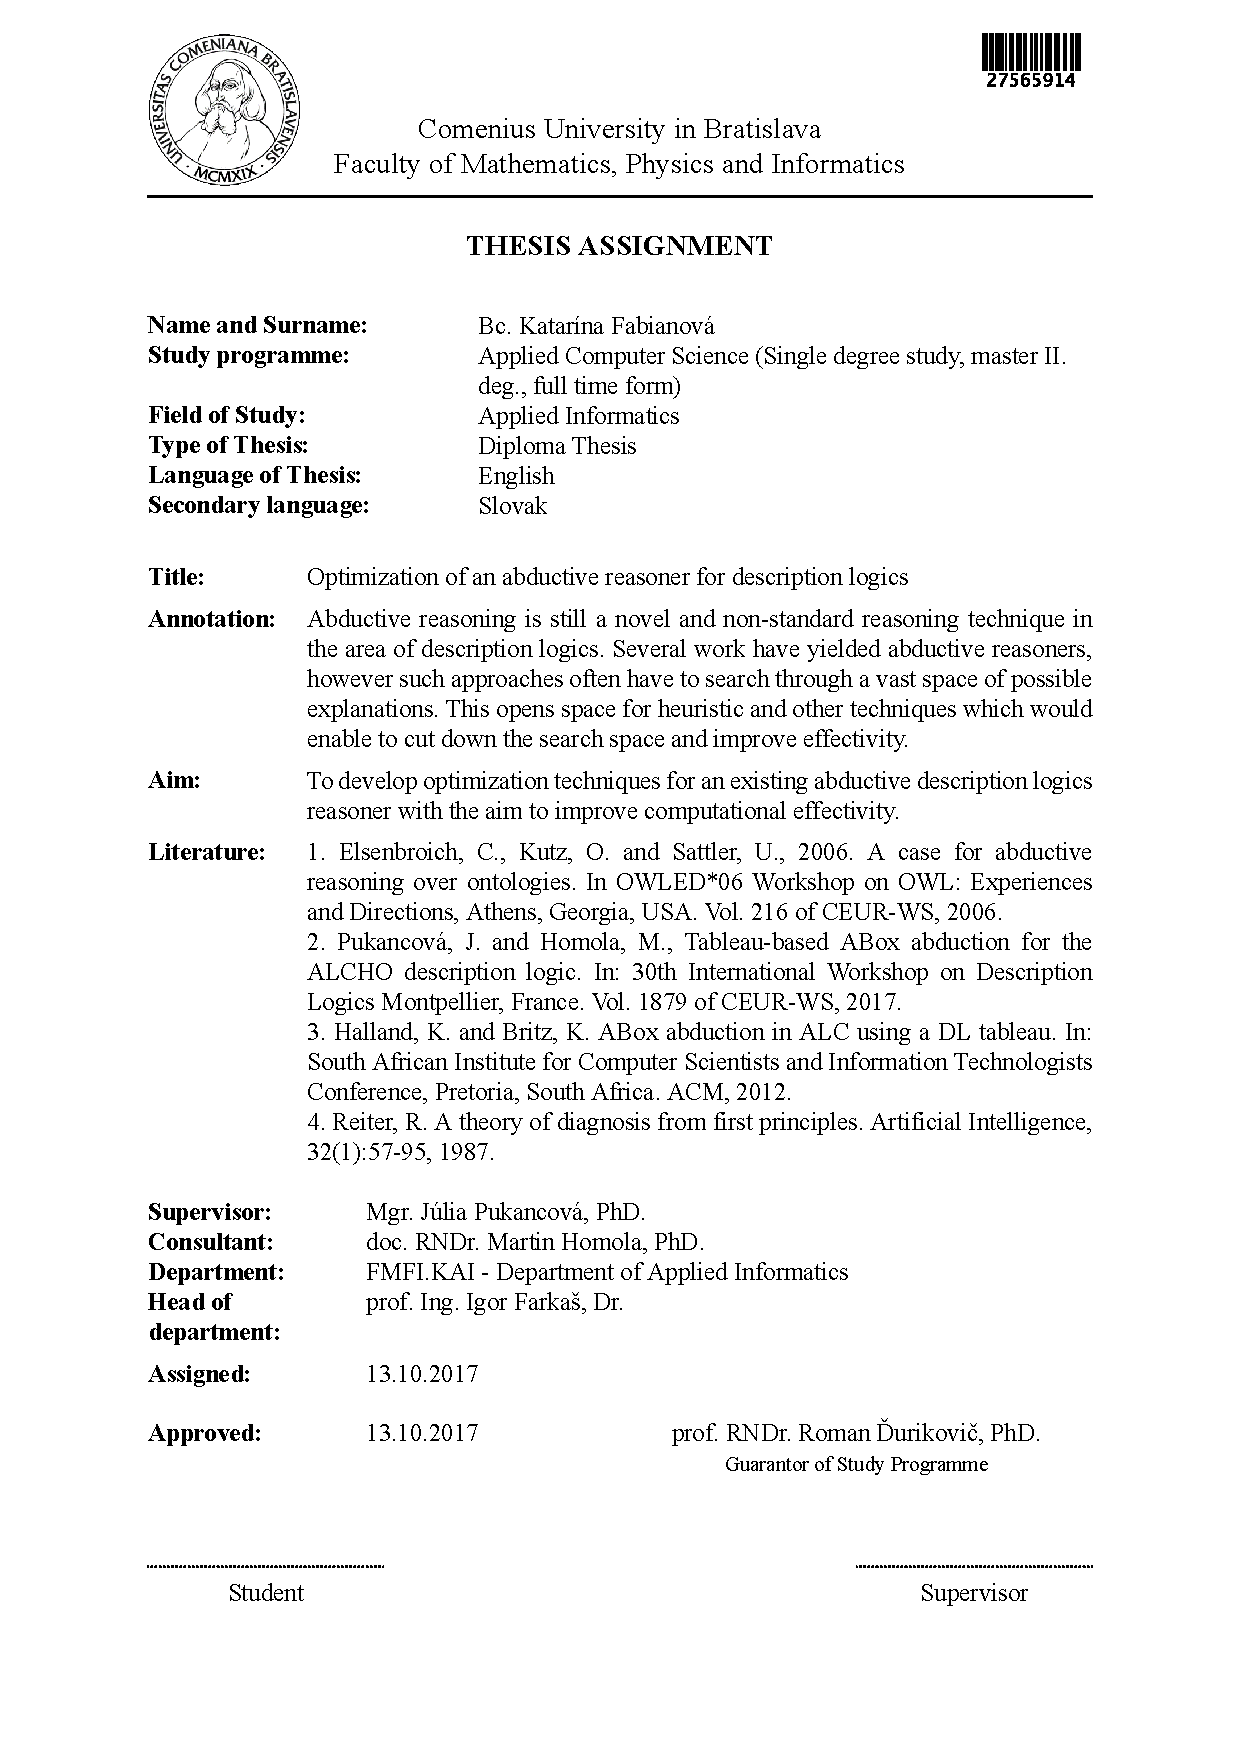
\includepdf[fitpaper=true, pages=-]{zadanieZaverecnejPraceEN.pdf}

\pagebreak

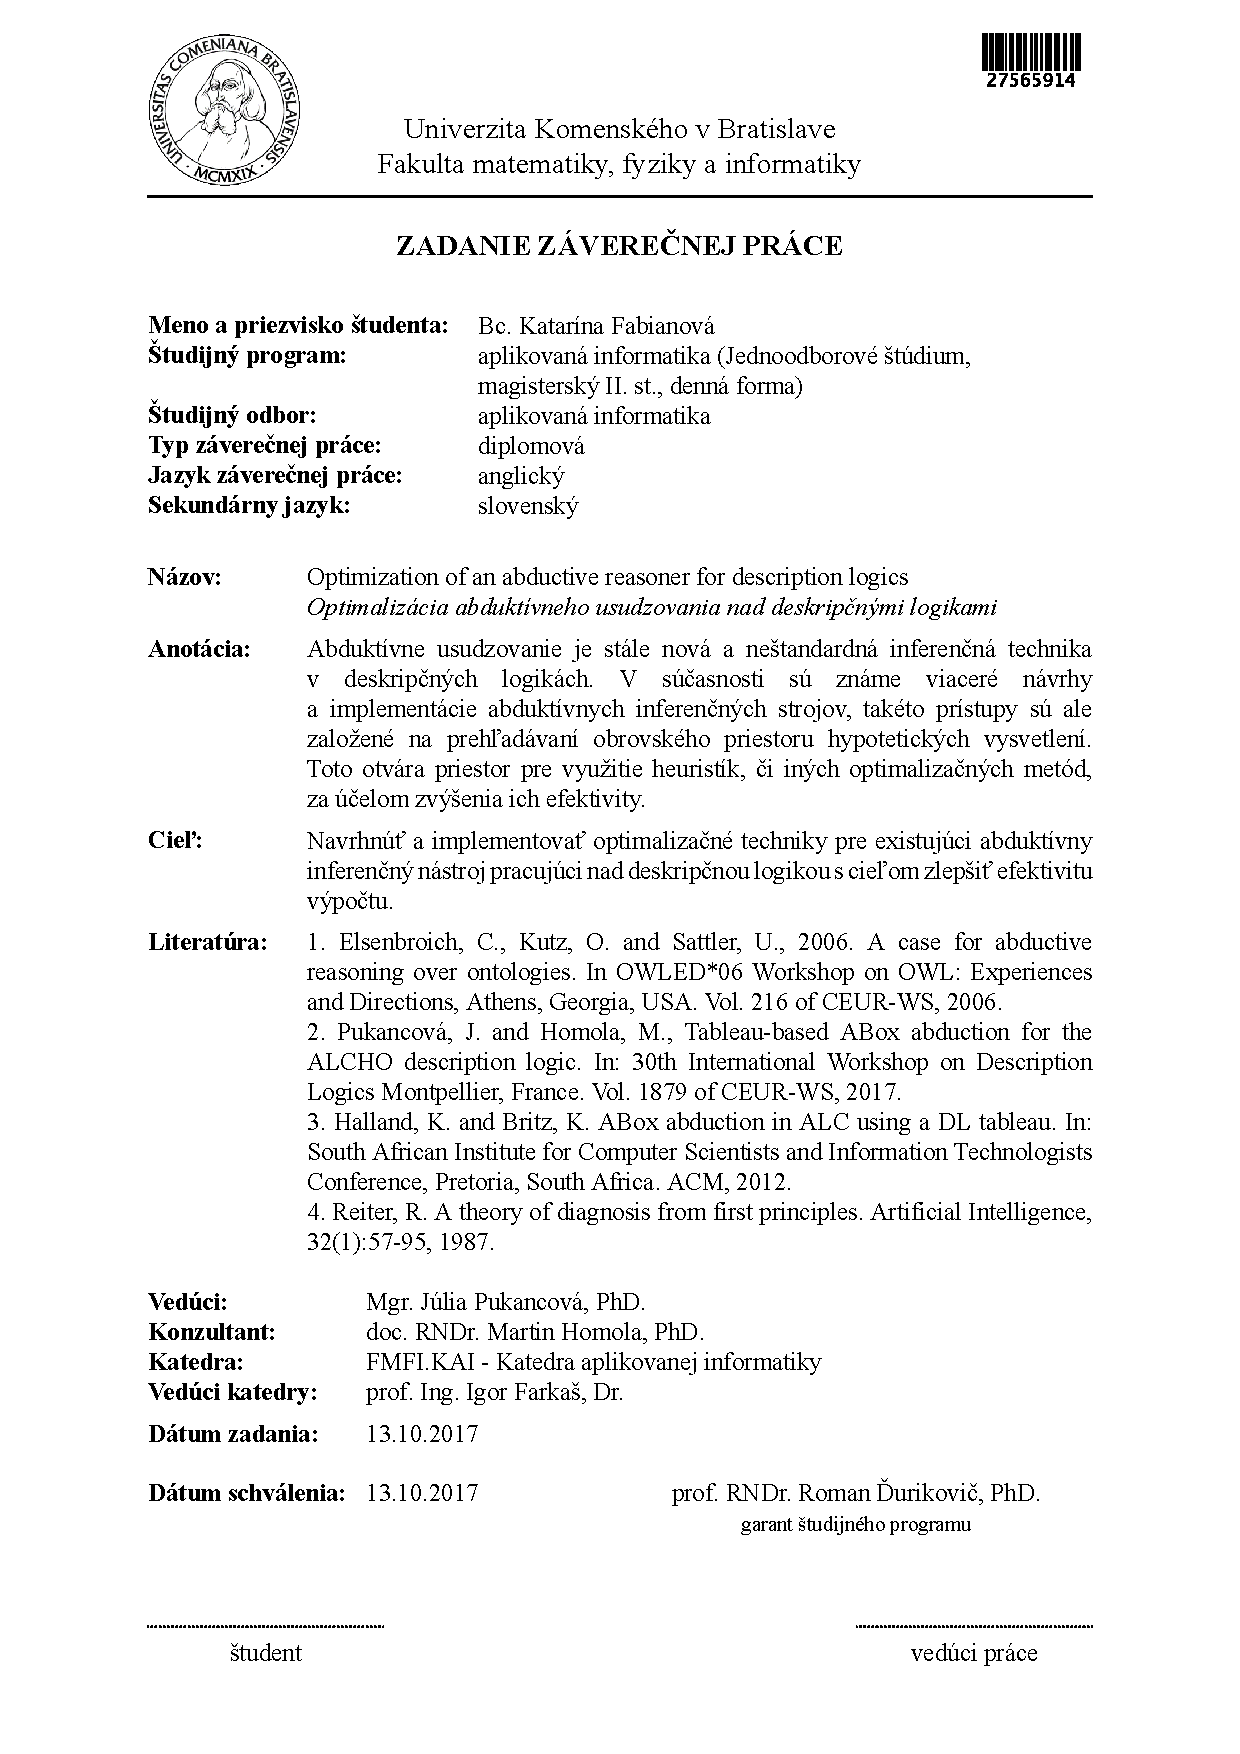
\includepdf[fitpaper=true, pages=-]{zadanieZaverecnejPraceSK.pdf}

\justify

\pagebreak
\thispagestyle{empty}
\vspace*{15cm}
{\large\bf Declaration of Honour \par}
\vspace{0.8cm}
{\large{I hereby declare that I wrote this Master thesis by myself only with the help of the referenced literature and with the help of my adviser and consultant.}} \par
\vspace{3cm}
{\large{Bratislava \hfill \textoverline{Bc. Katarína Fabianová}}}

\pagebreak
\thispagestyle{empty}
\par\vspace*{15cm}
{\large\bf \noindent Acknowledgements \par}
\vspace{0.8cm}
{\large{I would like to thank to my adviser Mgr. Júlia Pukancová, PhD. and to my consultant RNDr. Martin Homola, PhD. for their amazing help, valuable advice and for their guidance that helped me write this thesis.}}

\pagebreak
\thispagestyle{empty}
{\large\bf  \noindent Abstract \newline} 

Logical abduction is a form of logical reasoning where we are familiar with a knowledge base and an observation but we do not know the explanations. In this work we focus on ABox abduction in description logics. Our task is to optimize ABox abduction problem which purpose is to look for minimal explanations. We have implemented the Minimal Hitting Set algorithm and the MergeXPlain algorithm. We have tested our implementations of these approaches and compared their execution times and number of found explanations in the evaluation. We have evaluated two cases, the first one searches only for minimal explanations of size one, the second one searches for all possible minimal explanations. We have come to the conclusions that the Minimal Hitting Set is quicker if we want only explanations of size one. The MergeXPlain algorithm is much more efficient than the Minimal Hitting Set algorithm in the second case but we cannot guarantee that it finds all minimal explanations. \newline

\noindent \textbf{Key words:}
Abduction, Description logics, Minimal Hitting Set, MergeXPlain

\pagebreak
\thispagestyle{empty}
{\large\bf  \noindent Abstrakt \newline} 

Logická abdukcia je typ logického odvodzovania, kde sme oboznámení s bázou znalostí a pozorovaním, ale nepoznáme vysvetlenia. V tejto práci sa venujeme ABox abdukcii v deskripčných logikách. Našou úlohou je optimalizovať problém ABox abdukcie, ktorej cieľom je nájsť minimálne vysvetlenia. Implementovali sme Minimal Hitting Set algoritmus a MergeXPlain algoritmus. Otestovali sme našu implementáciu oboch prístupov a porovnali sme ich čas vykonávania a počet nájdených vysvetlení. Vyhodnocovali sme dva prípady, prvý hľadá iba vysvetlenia veľkosti jedna, druhý prípad hľadá všetky možné minimálne vysvetlenia. Prišli sme k záveru, že Minimal Hitting Set algoritmus je rýchlejší, ak hľadáme iba vysvetlenia veľkosti jedna. MergeXPlain algoritmus je ale oveľa efektívnejší časovo v druhom prípade, ale nevieme zaručiť, že nájde všetky minimálne vysvetlenia. \newline

\noindent \textbf{Kľúčové slová:}
Abdukcia, Deskripčné logiky, Minimal Hittting Set, MergeXPlain

\pagebreak
\thispagestyle{empty}
\tableofcontents
\thispagestyle{empty}

\pagebreak
\thispagestyle{empty}
\listoffigures

\pagebreak
\setcounter{page}{1}
\section{Introduction}
Ontologies (\cite{staabHandbookOntology}) describe a specific domain in a formal language. They characterize hierarchies and relationships between classes in given domain. One of the most important languages to represent ontologies is the family of description logics. There are many description logics and each one of them has a different expressivity. In our thesis we work with $\mathcal{ALC}$ DL (\cite{schmidt1991attributive}).

In logic we study three ways of inference, deduction, induction and abduction. Logical abduction (\cite{peirce}) is a type of logical reasoning where we are familiar with a theory and an effect but we are interested in explanations that, together with the theory, would imply the effect. In ABox abduction task (\cite{Elsenbroich2006}) we know theory as the knowledge base, effect as the observation and we look for explanations which are data. We look only for minimal explanations.

The purpose of our thesis is to optimize ABox abduction task. Previous solution to the ABox abduction task (\cite{pukancovaPreliminaryReport}) is correct but it has exponential time complexity and we want to propose a solution that would be optimized with an emphasis placed on time. Previous solution uses the Minimal Hitting Set algorithm (\cite{reiterHS}) to solve the ABox abduction task. We want to compare our implementation of the Minimal Hitting Set algorithm with our implementation of the MergeXPlain algorithm (\cite{MXP}). The MergeXPlain algorithm looks for conflicts that could be our minimal explanations. We want to find out if we can use the MergeXPlain algorithm in our situation and how it could improve time complexity.

We have implemented both approaches in our thesis successfully. Our implementation was tested and evaluated whereby the evaluation was focused on two situations. The first situation is when we look only for minimal explanations of size one and the second situation is when we look for all the minimal explanations. The first situation showed that the Minimal Hitting Set algorithm is quicker but the MergeXPlain is also usable for this case. The second situation showed that the MergeXPlain algorithm cannot always find all minimal explanations but it can find its subset that is often equal to the set of all minimal explanations.

At first we will introduce description logics and abduction. Then we will present the theory of the Minimal Hitting Set algorithm and the MergeXPlain algorithm. After theory we will describe our approach with theses two algorithms and then we evaluate results from experiments.


\pagebreak
\section{Description Logics}
Description logics (DLs) are a family of knowledge representation formalism. Each description logic has different expressivity. Every expressivity is expressed with a unique set of constructors. We will work with $\mathcal{ALC}$, $\mathcal{EL}$ and $\mathcal{EL}${+}{+} DL. Each description logic has its own syntax and semantics. In this chapter we will introduce syntax and semantics \citep{Rudolph2011} for each DL that we will be working with.

\subsection{$\mathcal{ALC}$ DL}
$\mathcal{ALC}$ DL (\cite{schmidt1991attributive}) is a DL which is more expressive than $\mathcal{EL}$ and $\mathcal{EL}{+}{+}$ DL. $\mathcal{ALC}$ is less expressive than many other DLs. $\mathcal{ALC}$ stands for Attributive (Concept) Language with Complements. It means that not only complement of atomic concept is allowed but also a complement of complex concept is allowed.

\subsubsection{$\mathcal{ALC}$ Syntax}
$\mathcal{ALC}$ description logic consists of three mutually disjoint sets. These sets (Definition~\ref{def:DLVocabulary}) represent the whole vocabulary that is used by $\mathcal{ALC}$ DL.

\begin{definition}{\textbf{DL vocabulary}}
	\label{def:DLVocabulary}
	
	DL vocabulary contains all symbols we use in concepts and the knowledge base. It consists of three mutually disjoint sets: $N_{I}$, $N_{C}$ and $N_{R}$. 
	
	\begin{table}[H]
		\centering
		\begin{tabular}{c}
			$ \textbf{Set of individuals:} \text{ } N_{I} = \{a,b,c...\} $ \\
			\addlinespace[0.4cm]
			$ \textbf{Set of concepts:} \text{ } N_{C} = \{A,B,C...\} $ \\
			\addlinespace[0.4cm]
			$ \textbf{Set of roles:} \text{ } N_{R} = \{R_{1},R_{2},R_{3},...\} $			
		\end{tabular}
	\end{table}		
		
\end{definition}

\begin{example}{\textbf{DL vocabulary}}
	
	\begin{table}[H]
		\centering
		\begin{tabular}{c}
			$ N_{I} = \{ jack, john, jane \} $ \\
			\addlinespace[0.4cm]
			$ N_{C} = \{ Person, Mother, Father \} $ \\
			\addlinespace[0.4cm]
			$ N_{R} = \{ hasChild, likes, owns \} $
		\end{tabular}
	\end{table}
\end{example}

$\mathcal{ALC}$ DL deals with individuals and concepts. An individual is a concrete instance of a concept. Concept is a class that defines some entity. Concept can be atomic or complex. Atomic concept is not constructed with any constructor. On the contrary, complex concept is created from constructors and other concepts.

\begin{definition}{\textbf{Complex concept}}
	\label{def:complexConcept}
	
	Concepts are recursively constructed as the smallest set of expressions of the forms:

	\begin{table}[H]
		\centering
		\begin{tabular}{c}
			$ C,D ::= A | \neg C | C \sqcap D | C \sqcup D | \exists R.C | \forall R.C $
		\end{tabular}
	\end{table}

	where $A \in N_{C}$, $R \in N_{R}$, and C, D are concepts.
\end{definition}

Practical usage of Definition ~\ref{def:complexConcept} is shown in Example~\ref{example:complexConcept}.

\begin{example}{\textbf{Complex concept}}
	\label{example:complexConcept}
	
	\begin{table}[H]
		\centering
		\begin{tabular}{c}
			$ \neg Mother $ \\
			\addlinespace[0.4cm]
			$ Mother \sqcup Father $ \\
			\addlinespace[0.4cm]			
			$ \exists hasChild.Person $ \\
			\addlinespace[0.4cm]			
			$ \forall likes.Food $ \\
		\end{tabular}
	\end{table}
\end{example}

Complex concept uses following constructors: $\neg$, $\sqcup$, $\sqcap$, $\exists$ and $\forall$. Constructor $\neg$ is negation, constructor $\sqcup$ is or and constructor $\sqcap$ is and. Constructors $\exists$ is existential restriction and $\forall$ is called value restriction.

There are two concepts that are always in ontology. $\top$ (top) stays for everything. Each concept belongs under $\top$ which means that each concept is on left side of subsumption if on right side is only $\top$. Second concept is $\bot$ (bottom) and it stays for nothing which means that each concept is on the right side of subsumption if there is only $\bot$ on the left side. Formally these two concepts can be written as we see in Definition~\ref{def:topBottom}.

\begin{definition}{\textbf{Top and Bottom}}
	\label{def:topBottom}
	
	\begin{table}[H]
		\centering
		\begin{tabular}{c}
			$ \top \equiv A \sqcup \neg A $ \\
			\addlinespace[0.4cm]
			$ \bot \equiv A \sqcap \neg A $
		\end{tabular}
	\end{table}
\end{definition}

$\mathcal{ALC}$ description logic uses axioms in order to model some situation. Ontology \citep{staabHandbookOntology} is used to formally describe these axioms. The purpose of ontology is to describe relationships between entities in a formal language. Every ontology has its own knowledge base. Knowledge base is a set of TBox axioms and ABox axioms. Ontology is described by knowledge base. Knowledge base is defined in Definition~\ref{def:knowledgeBase}.

\begin{definition}{\textbf{Knowledge base}}
	\label{def:knowledgeBase}
	
	Knowledge base ($\mathcal{KB}$) is an ordered pair of \textit{TBox} $\mathcal{T}$ and \textit{ABox} $\mathcal{A}$.
\end{definition}

An example for knowledge base is shown in Example ~\ref{example:knowledgeBase}.

\begin{example}{\textbf{Knowledge base}}
	\label{example:knowledgeBase}
	\[ 
	\mathcal{KB} = \left\{
	\begin{tabular}{c c}
	$Professor \sqcup Scientist \sqsubseteq Academician$ \\
	$AssocProfessor \sqsubseteq Professor$ \\
	$jack : Academician$ \\
	$jane : Scientist$ \\
	$john : Professor$ \\	
	\end{tabular}
	\right \}
	\]
\end{example}

There are two types of axioms, the first is TBox (Definition~\ref{def:tbox}) and the second one is ABox (Definition~\ref{def:abox}). In TBox the subsumption symbol ($\sqsubseteq$) is used. Let us explain this symbol on an example $Mother \sqsubseteq Parent$. $Mother$ is always a $Parent$ but $Parent$ does not always have to be a $Mother$. TBox represents axioms that model ontology. Each axiom explains the relationship between entities in this axiom.

\begin{definition}{\textbf{TBox}}
	\label{def:tbox}
	
	A TBox $\mathcal{T}$ is a finite set of GCI axioms $\phi$ of the form:
	
	\begin{table}[H]
		\centering
		\begin{tabular}{c}
			$ \phi ::= C \sqsubseteq D $
		\end{tabular}
	\end{table}
			
	where C, D are any concepts.
\end{definition}

\begin{example}{\textbf{TBox}}
	\[ 
	\mathcal{T} = \left\{
	\begin{tabular}{c c}
	$Professor \sqcup Scientist \sqsubseteq Academician$ \\
	$AssocProfessor \sqsubseteq Professor$ \\
	\end{tabular}
	\right \}
	\]
\end{example}

ABox, on the other side, does not model ontology but creates a database of facts. It contains a set of assertion axioms that can be called facts. Fact is a direct assertion of an individual to a concept.

\begin{definition}{\textbf{ABox}}
	\label{def:abox}
	
    An ABox $\mathcal{A}$ is a finite set of assertion axioms $\phi$ of the form:
	\begin{table}[H]
		\centering
		\begin{tabular}{c}
			$ \phi ::= a:C | a,b:R $
		\end{tabular}
	\end{table}
	where $a,b \in N_{I}$, $R \in N_{R}$ and C is any concept.
\end{definition}

\begin{example}{\textbf{ABox}}
	\[ 
	\mathcal{A} = \left\{
	\begin{tabular}{c c}
	$jack : Academician$ \\
	$jane : Scientist$ \\
	$john : Professor$ \\
	\end{tabular}
	\right \}
	\]
\end{example}

To gain a better understanding of $\mathcal{ALC}$ DL, we can translate sentences into $\mathcal{ALC}$ description logic (Example~\ref{example:sentences}).

\begin{example}{\textbf{ABox}}
	\label{example:sentences}
	
	\begin{table}[H]
		\centering
		\begin{tabular}{c c}
			Everybody who is sick, is not happy & $Sick \sqsubseteq \neg Happy$ \\ \addlinespace[0.4cm]
			Cat and dogs are animals. & $Cat \sqcup Dog \sqsubseteq Animal$ \\ \addlinespace[0.4cm]
			Every person owns a house. & $Person \sqsubseteq \exists owns.House$ \\	\addlinespace[0.4cm]
		\end{tabular}		
	\end{table}
\end{example}

\subsubsection{$\mathcal{ALC}$ Semantics}
An interpretation is a pair of a domain and an interpretation function. The domain is a set of values that represents concepts in the interpretation (Definition~\ref{def:interpretation}). The result of interpretation function is different for individuals, concepts and roles. If we use the interpretation function on an individual, the result is an element from the domain. If we use it on the concepts, the result is a set of elements from the domain. If we use it on the roles, the result is a set of pairs of elements from the domain.

\begin{definition}{\textbf{Interpretation}}
	\label{def:interpretation}

	An interpretation of a given knowledge base $\mathcal{KB} = (\mathcal{T}, \mathcal{A})$ is a pair $\mathcal{I} = (\Delta^{\mathcal{I}}, \cdot ^{\mathcal{I}})$ which contains a domain $\Delta^{\mathcal{I}}$ and an interpretation function $\cdot ^{\mathcal{I}}$.	
	Domain cannot be empty.
		
	The interpretation function is following:
	
	\begin{table}[H]
		\centering
		\begin{tabular}{c c}
			$ a^{\mathcal{I}} \in \Delta^{\mathcal{I}} \text{ } \forall a \in N_{I} $ \\ \addlinespace[0.4cm]
			 $A^{\mathcal{I}} \subseteq \Delta^{\mathcal{I}} \text{ } \forall A \in N_{C} $ \\
			\addlinespace[0.4cm]
			$ R^{\mathcal{I}} \subseteq \Delta^{\mathcal{I}} \times \Delta^{\mathcal{I}} \text{ } \forall R \in N_{R} $ \\
		\end{tabular}		
	\end{table}

\newpage	
	The interpretation of complex concepts is recursively defined:

	\begin{table}[H]
		\centering
		\begin{tabular}{c c}
			$ \neg C^{\mathcal{I}} = \Delta^{\mathcal{I}} \backslash C^{\mathcal{I}} $ \\ \addlinespace[0.4cm]
			$ C \sqcap D^{\mathcal{I}} = C^{\mathcal{I}} \cap D^{\mathcal{I}} $ \\
			\addlinespace[0.4cm]
			$ C \sqcup D^{\mathcal{I}} = C^{\mathcal{I}} \cup D^{\mathcal{I}} $ \\
			\addlinespace[0.4cm]
			$ \exists R.C^{\mathcal{I}} = \{ x \in \Delta^{\mathcal{I}} | \exists y \in \Delta^{\mathcal{I}} : \langle x,y \rangle \in R^{\mathcal{I}} \land y \in C^{\mathcal{I}} \} $ \\
			\addlinespace[0.4cm]
			$ \forall R.C^{\mathcal{I}} = \{ x \in \Delta^{\mathcal{I}} | \forall y \in \Delta^{\mathcal{I}} : \langle x,y \rangle \in R^{\mathcal{I}} \rightarrow y \in C^{\mathcal{I}} \} $								
		\end{tabular}		
	\end{table}
		
\end{definition}

\begin{example}{\textbf{Interpretation}}
	\[ 
	\mathcal{KB} = \left\{
	\begin{tabular}{c c}
	$Professor \sqcup Scientist \sqsubseteq Academician$ \\
	$AssocProfessor \sqsubseteq Professor$ \\
	$jack : Academician$ \\
	\end{tabular}
	\right \}
	\]
	
	\begin{table}[H]
		\centering
		\begin{tabular}{c}
			$ \mathcal{I} = (\Delta ^{\mathcal{I}}, \cdot^{\mathcal{I}}) $ \\
			\addlinespace[0.4cm]
			$ \Delta ^{\mathcal{I}} = \{ P,S,A,AP \} $ \\
			\addlinespace[0.4cm]
			$ Professor^{\mathcal{I}} = \{P\} $ \\
			\addlinespace[0.4cm]
			$ Scientist^{\mathcal{I}} = \{S\} $ \\
			\addlinespace[0.4cm]
			$ Academician^{\mathcal{I}} = \{A\} $ \\
			\addlinespace[0.4cm]
			$ AssocProfessor^{\mathcal{I}} = \{AP\} $ \\
			\addlinespace[0.4cm]
			$ jack^{\mathcal{I}} = A $
		\end{tabular}
	\end{table}

\end{example}

The interpretation satisfies (Definition~\ref{def:satisfaction}) an axiom according to its type. We know three types of axioms. The first is an axiom from TBox, the second one is an assertion axiom to a concept and the third one is an assertion to a role.

\newpage
\begin{definition}{\textbf{Satisfaction $\models$}}
	\label{def:satisfaction}

	Given an axiom $\phi$, an interpretation $\mathcal{I} = (\Delta^{\mathcal{I}}, \cdot ^{\mathcal{I}})$ satisfies $\phi (\mathcal{I} \models \phi)$ depending on its type:
	
	\begin{table}[H]
		\centering
		\begin{tabular}{c}
			$ \mathcal{I} \models C \sqsubseteq D \text{ iff } C^{\mathcal{I}} \subseteq D^{\mathcal{I}} $ \\
			\addlinespace[0.4cm]
			$ \mathcal{I} \models a:C \text{ iff } a^{\mathcal{I}} \in C^{\mathcal{I}} $ \\
			\addlinespace[0.4cm]
			$ \mathcal{I} \models a,b:R \text{ iff } \langle a^{\mathcal{I}}, \in b^{\mathcal{I}} \rangle \in R^{\mathcal{I}} $
		\end{tabular}
	\end{table}

\end{definition}

Finding a model (an interpretation satisfying $\mathcal{KB}$, Definition~\ref{def:model}) is crucial for consistency checking. If we find at least one model, the knowledge base $\mathcal{KB}$ is consistent. We can have more models for one knowledge base. In Example~\ref{example:model} there are two showed models but there can be more models. 

\begin{definition}{\textbf{Model}}
	\label{def:model}

	An interpretation $\mathcal{I} = \langle \Delta^{\mathcal{I}}, \cdot ^{\mathcal{I}}  \rangle$ is a model of a DL knowledge base $\mathcal{KB} = (\mathcal{T}, \mathcal{A})$ iff $\mathcal{I}$ satisfies every axiom in TBox $\mathcal{T}$ and ABox $\mathcal{A}$.
\end{definition}

\begin{example}{\textbf{Model}}
	\label{example:model}
	\[ 
	\mathcal{KB} = \left\{
	\begin{tabular}{c c}
	$Professor \sqcup Scientist \sqsubseteq Academician$ \\
	$AssocProfessor \sqsubseteq Professor$ \\
	$jack : Academician$ \\
	\end{tabular}
	\right \}
	\]

	\begin{table}[H]
		\centering
		\begin{tabular}{c}
			$ \mathcal{I}_{1} = \{  \Delta^{\mathcal{I}} = \{ P,S,A,AP \}, $ \\
			\addlinespace[0.4cm]
			$ Professor^{\mathcal{I}} = \{P\}, Scientist^{\mathcal{I}} = \{S\}, Academician^{\mathcal{I}} = \{A\}, AssocProfessor^{\mathcal{I}} = \{AP\} $ \\
			\addlinespace[0.4cm]
			$ jack^{\mathcal{I}} = A \} $
		\end{tabular}
	\end{table}
		
	\begin{table}[H]
		\centering
		\begin{tabular}{c}
			$ \mathcal{I}_{2} = \{  \Delta^{\mathcal{I}} = \{ A \}, $ \\
			\addlinespace[0.4cm]
			$ Professor^{\mathcal{I}} = \{A\}, Scientist^{\mathcal{I}} = \{A\}, Academician^{\mathcal{I}} = \{A\}, AssocProfessor^{\mathcal{I}} = \{A\} $ \\
			\addlinespace[0.4cm]
			$ jack^{\mathcal{I}} = A \} $
		\end{tabular}
	\end{table}

\end{example}

\begin{definition}{\textbf{Consistency}}
	
	A knowledge base $\mathcal{KB}$ is consistent iff $\mathcal{KB}$ has at least one model $\mathcal{I}$.
\end{definition}

We are familiar with more decision problems, satisfiability, subsumption $(\sqsubseteq)$, equivalence ($\equiv$) and disjointness. Satisfiability means that concept is satisfiable in regard to $\mathcal{KB}$ if we can find such a model of a knowledge base for which holds that interpretation of that concept is not empty. Subsumption between two concepts must hold that interpretation of left-sided concept is a proper subset of interpretation of right-sided concept in each possible model of a knowledge base. Equivalence is similar to subsumption but the difference is that the interpretations of both concepts must be equal in each possible model of a knowledge base. Disjointness means that intersection of the interpretations of both concepts must be an empty set in each possible model of a knowledge base.

\begin{definition}{\textbf{Decision problems}}

	Given a DL $\mathcal{KB} = (\mathcal{T}, \mathcal{A})$, and two concepts C,D, we say that:

	\begin{itemize}
		\item $C \text{ is satisfiable w.r.t. } \mathcal{KB} \text{ iff there is such a model } \mathcal{I} \text{ of } \mathcal{KB} \text{ for which holds that } \newline C^{\mathcal{I}} \neq \emptyset;$

		\item $C \text{ is subsumed by D w.r.t. } \mathcal{KB} \text{ (denoted } \mathcal{KB} \models C \sqsubseteq D) \text{ iff } C^{\mathcal{I}} \subseteq D^{\mathcal{I}} \text{ in every} \newline \text{model } \mathcal{I} \text{ of } \mathcal{KB};$

		\item $\text{C and D are equivalent w.r.t. } \mathcal{KB} \text{ (denoted } \mathcal{KB} \models C \equiv D) \text{ iff } C^{\mathcal{I}} = D^{\mathcal{I}} \text{ in every} \newline \text{model } \mathcal{I} \text{ of } \mathcal{KB};$
		
		\item $\text{C and D are disjoint w.r.t. } \mathcal{KB} \text{ iff } C^{\mathcal{I}} \cap D^{\mathcal{I}} = \emptyset \text{ in every model } \mathcal{I} \text{ of } \mathcal{KB}.$		
	\end{itemize}
\end{definition}

If $\mathcal{KB} = \emptyset$ then we say that decision problems (satisfiability, subsumption, equivalence and disjointness) of concepts are defined in general by definition and we use notation such as we omit $\mathcal{KB} \models$ from the notation.

\subsection{DL Tableau Algorithm}
Following definitions \citep{baaderHandbook} describe rules and terms that are used by this algorithm. DL Tableau algorithm proves satisfiability of a concept or checks consistency of a given knowledge base. By proving satisfiability the input for the algorithm is concept C and TBox $\mathcal{T}$. By checking consistency the input for the algorithm is a knowledge base $\mathcal{KB}$. If the knowledge base $\mathcal{KB}$ is consistent, then this knowledge base $\mathcal{KB}$ must have at least one model. In both versions of the algorithm it is held that each concept must be in NNF (negation normal form, Definition ~\ref{def:nnf}). Negation normal form is such a form that each negation is pushed in front of atomic concept inside a complex concept. 

\begin{definition}{\textbf{NNF}}
	\label{def:nnf}
	
	A concept C is in NNF (negation normal form) if and only if the complement constructor $\neg$ only occurs in front of atomic concept symbols inside C.
\end{definition}

\begin{example}{\textbf{NNF}}
	\begin{table}[H]
		\centering
		\begin{tabular}{c}
			$ nnf(\neg (C \sqcap D)) = \neg C \sqcup \neg D $ \\
			\addlinespace[0.4cm]
			$ nnf(\neg (C \sqcup D)) = \neg C \sqcap \neg D $ \\
			\addlinespace[0.4cm]
			$ nnf(\neg \exists R.C) = \forall R. \neg C $ \\
			\addlinespace[0.4cm]
			$ nnf(\neg \forall R.C) = \exists R. \neg C $
		\end{tabular}
	\end{table}
	
\end{example}

DL Tableau algorithm creates a CTree (Completion tree, Definition~\ref{def:ctree}). CTree proves whether model exists or not.

\begin{definition}{\textbf{Completion tree}}
	\label{def:ctree}

	A completion tree (CTree) is a triple T = (V, E, $\mathcal{L}$) where (V, E)
	is a tree and $\mathcal{L}$ is a labeling function which means that:
	$\mathcal{L}(x)$ is a set of concepts $\forall x \in V$ and
	$\mathcal{L}(\langle x, y \rangle )$ is a set of roles $\forall \langle x, y \rangle \in E$.	
\end{definition}

At first the algorithm creates node and initializes it with the input concept.
Then the algorithm applies tableau rules for given DL. If the algorithm applies each rule until any rule can be applied and it finds no clash, then the result is that the concept C is satisfiable w.r.t. $\mathcal{T}$. Children of a node are called successors or R-successors (Definition~\ref{def:successor}).

\begin{definition}{\textbf{Successor, R-successor}}
	\label{def:successor}

	Given a CTree T = (V,E, $\mathcal{L}$) and $x,y \in V$ we say that: 
	\begin{itemize}
		\item y is a successor of x iff $\langle x,y \rangle \in E$
		\item y is an R-successor of x iff $\langle x,y \rangle \in E$ and $R \in \mathcal{L}(\langle x,y \rangle)$.
	\end{itemize}
\end{definition}

A clash containing Ctree is such a tree that one branch of this tree contains a concept and simultaneously its negation, too. Clash is defined in Definition~\ref{def:clash}.

\begin{definition}{\textbf{Clash}}
	\label{def:clash}

	There is a clash in a CTree T = $(V,E, \mathcal{L})$ if and only iff for some $x \in V$ and for some concept C both $C \in \mathcal{L}(x)$ and $\neg C \in \mathcal{L}(x)$.
\end{definition}

\begin{example}{\textbf{Clash}}
	\[ \mathcal{L}(s_{0}) = \{ C, D, \neg D \} \]
\end{example}

\begin{definition}{\textbf{Clash-free CTree}}

A CTree T = $(V,E, \mathcal{L})$ is clash-free iff none of the nodes in V contains a clash.
\end{definition}

There can be a situation that some concept can lead to infinite looping and algorithm would never stop. This situation is called blocking (Definition~\ref{def:blocking}). An example for that is: $Person \sqsubseteq \exists hasParent.Person$. That is why the algorithm uses Blocking rule.

\begin{definition}{\textbf{Blocking}}
	\label{def:blocking}
	
	Given a CTree $T = (V, E, \mathcal{L})$ a node $x \in V$ is blocked if it has an ancestor $y$ such that: either $\mathcal{L}(x) \subseteq \mathcal{L}(y)$ or $y$ is blocked.
\end{definition}

DL Tableau algorithm proves concept satisfiability in regard of TBox (Definition~\ref{def:conceptSatisfiability}). Input for DL Tableau algorithm is concept C and TBox $\mathcal{T}$. Output is a boolean value which is true if concept C is satisfiable w.r.t. $\mathcal{T}$, false otherwise.

\begin{definition}{\textbf{Algorithm -- Concept satisfiability}}	
	\label{def:conceptSatisfiability}

	\textbf{Input:} concept C and $\mathcal{T}$ in NNF \newline
	\indent \textbf{Output:} answers whether concept C is satisfiable w.r.t. $\mathcal{T}$ or not \newline
	\indent \textbf{Steps:}
	\begin{enumerate}
		\item Initialize a new CTree T := $(\{s_{0}\}, \emptyset, \{s_{0} \rightarrow \{C\}\})$;
		\item Apply tableau rules for TBoxes while at least one rule is applicable;
		\item Answer "C is satisfiable w.r.t. $\mathcal{T}$" if T is clash-free. Otherwise answer "C is unsatisfiable w.r.t. $\mathcal{T}$".
	\end{enumerate}
\end{definition}

\begin{definition}{\textbf{$\mathcal{ALC}$ tableau rules for TBoxes}}
	\begin{itemize}
		\item $\sqcap-rule:$ if $C_{1} \sqcap C_{2} \in \mathcal{L}(x)$ and $x \in V$ and $\{ C_{1}, C_{2} \} \not \subseteq \mathcal{L}(x)$ and x is not blocked then $\mathcal{L}(x) = \mathcal{L}(x) \cup \{ C_{1}, C_{2} \}$
		
		\item $\sqcup-rule:$ if $C_{1} \sqcup C_{2} \in \mathcal{L}(x)$ and $x \in V$ and $ \{ C_{1}, C_{2} \} \cap \mathcal{L}(x) = \emptyset$ and x is not blocked then either $\mathcal{L}(x) = \mathcal{L}(x) \cup \{ C_{1} \}$ or $\mathcal{L}(x) = \mathcal{L}(x) \cup \{ C_{2} \}$
		
		\item $\forall-rule:$ if $\forall R.C \in \mathcal{L}(x)$ and $x,y \in V$ and y is R-successor of x and $C \not \in \mathcal{L}(y)$ and x is not blocked then $\mathcal{L}(y) = \mathcal{L}(y) \cup \{ C \}$
		
		\item $\exists-rule:$ if $\exists R.C \in \mathcal{L}(x)$ and $x \in V$ with no R-successor y and $C \in \mathcal{L}(y)$ and x is not blocked then $\mathcal{V} = \mathcal{V} \cup \{ z \}, \mathcal{L}(z) = \{ C\}$ and $\mathcal{L}( \langle x, z \rangle ) = \{ R \}$
		
		\item $\mathcal{T}-rule:$ if $C_{1} \sqsubseteq C_{2} \in \mathcal{T}$ and $x \in V$ and nnf$(\neg C_{1} \sqcup C_{2}) \not \in \mathcal{L}(x)$ and x is not blocked then $\mathcal{L}(x) = \mathcal{L}(x) \cup \{ nnf(\neg C_{1} \sqcup C_{2}) \}$
	\end{itemize}
\end{definition}	

Knowledge base is a pair of a TBox and an Abox and yet only a TBox was mentioned in connection with the DL Tableau algorithm. If we also have a given ABox, the algorithm must be modified. The algorithm checks no longer concept satisfiability w.r.t. $\mathcal{T}$ but it checks the consistency of a given $\mathcal{KB}$. The same condition holds for the result as in proving concept satisfiability. If there is a found clash, the knowledge base is not consistent; otherwise the knowledge base is consistent (Definition~\ref{def:consistency}). The difference between the first version of this algorithm is that here, named nodes are used. Name of the node is an instance of a concept that comes from ABox. 

\begin{definition}{\textbf{Algorithm -- Consistency checking}}
	\label{def:consistency}

\textbf{Input:} $\mathcal{KB} = (\mathcal{T}, \mathcal{A})$ in NNF \newline
\indent \textbf{Output:} answers whether $\mathcal{KB}$ is consistent or not \newline
\indent \textbf{Steps:}
\begin{enumerate}
	\item Initialize a CTree T as follows:
		\begin{itemize}
			\item $V := \{ a \text{ } | \text{ individual a occurs in } \mathcal{A} \}$;
			\item $E := \{ \langle a,b \rangle \text{ } | \text{ } a,b : R \in \mathcal{A} \text{ for some role R} \}$;
			\item $\mathcal{L}(a) := \{ nnf(E) \text{ } | \text{ } a:E \in \mathcal{A}\} \text{ for all } a \in V$; \newline
			$\mathcal{L}(\langle a,b \rangle) := \{ R \text{ } | \text{ } a,b:R \in \mathcal{A}\} \text{ for all } \langle a,b \rangle \in E$;
		\end{itemize}
	\item Apply tableau rules for TBoxes while at least one rule is applicable;
	\item Answer "$\mathcal{KB}$ is consistent" if T is clash-free. Otherwise answer "$\mathcal{KB}$ is inconsistent".
\end{enumerate}

\end{definition}

Let us introduce an Example~\ref{example:dlTableau} where we know a knowledge base $\mathcal{KB}$. DL Tableau algorithm checks if knowledge base is consistent or not.

\begin{example}{(\textbf{DL Tableau algorithm})}
	\label{example:dlTableau}
	\[ 
	\mathcal{KB} = \left\{
	\begin{tabular}{c c}
	$Student \sqsubseteq \exists attends.MathCourse$ \\
	$MathCourse \sqsubseteq Course$ \\
	$jack : Student$ \\
	\end{tabular}
	\right \}
	\] \\
\end{example}

\begin{center}
	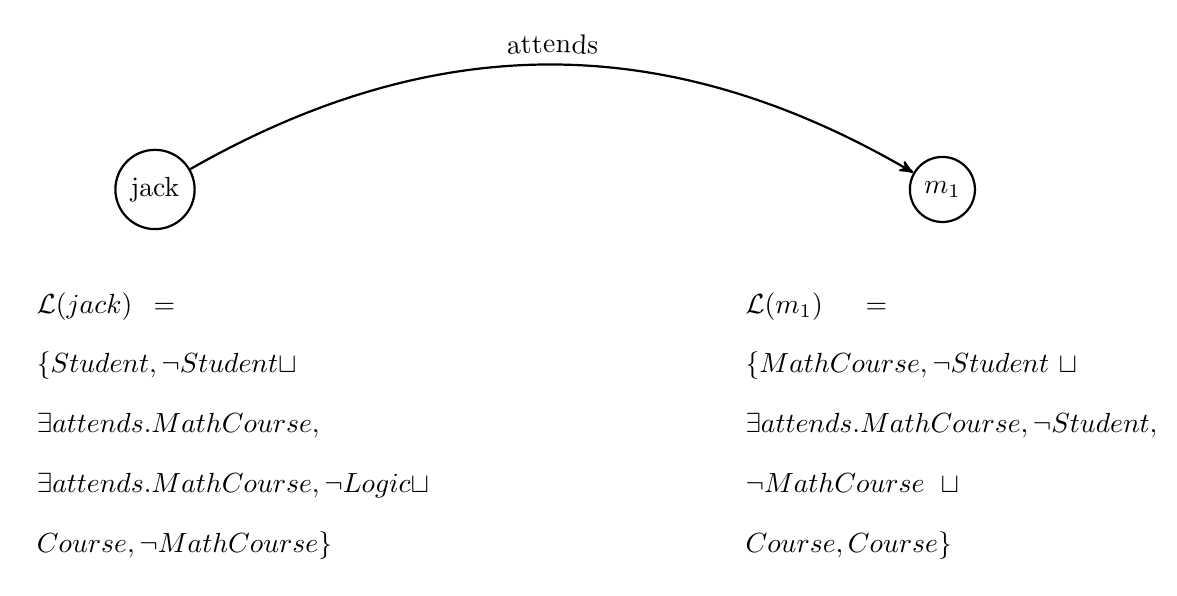
\begin{tikzpicture}[->,>=stealth',auto,node distance=10cm,
	thick,main node/.style={circle, draw}]
	
	\node[main node] (1) {jack};
	\node[main node] (2) [right of=1] {$m_{1}$};
	
	\def\myshift#1{\raisebox{1ex}}
	
	\draw [thick, ->, postaction={decorate, decoration={text along path, text align=center, text={|\myshift|attends}}}] (1) to [bend left=30] (2);
	
	\node[text width=3cm] at (0,-3) 
	{$\mathcal{L}(jack) = \{ Student, \neg Student \sqcup \exists attends.MathCourse, \newline \exists attends.MathCourse, \neg Logic \sqcup Course, \neg MathCourse \}$};		

	\node[text width=5cm] at (10,-3) 
	{$\mathcal{L}(m_{1}) = \{ MathCourse, \neg Student \sqcup \exists attends.MathCourse, \neg Student, \newline \neg MathCourse \sqcup Course, Course \}$};			
	\end{tikzpicture}
\end{center}

The algorithm starts with the ABox assertion axioms. It selects the axiom $jack : Student$. At first it creates a node $jack$ with its label $\mathcal{L}(jack)$. From the assertion axiom $jack : Student$ algorithm knows that jack is a Student and adds the concept $Student$ to the label $\mathcal{L}(jack)$. Then the algorithm chooses another axiom from the knowledge base. There are no more assertion axioms, so it starts with the axioms from TBox. It takes $Student \sqsubseteq \exists attends.MathCourse$. It must convert it into the negation normal form which is $\neg Student \sqcup \exists attends.MathCourse$. The algorithm applies $\sqcup-rule$. According to this rule it must choose $\exists attends.MathCourse$, otherwise there would be a clash. Now it has to apply $\exists - rule$ so a new node $l_{1}$ will be created with its label $\mathcal{L}(m_{1})$. Concept $MathCourse$ will be added into this label. Let us go back to the $jack$ node. The algorithm has to finish adding all axioms of TBox form. It will add the second axiom from the knowledge base in negation normal form as $\neg MathCourse \sqcup Course$. Now it does not matter which one the algorithm chooses if $Course$ or $\neg MathCourse$ because any of these two does not cause a clash. Now the algorithm goes back to the $m_{1}$ node and continues to add axioms from the knowledge base similarly as in the node $jack$. It starts with axiom $\neg Student \sqcup \exists attends.MathCourse$, it will choose the first one $\neg Student$. Then continues with axiom $\neg MathCourse \sqcup Course$. It cannot choose $\neg MathCourse$ because there would be immediately a clash. So it chooses $Course$.

The created tree contains two nodes ($jack$ and $m_{1}$) and one edge between them. The edge represents that $jack$ attends some MathCourse $m_{1}$. There is not any instance of a concept $MathCourse$ so the node $m_{1}$ does not represent a concrete instance of the concept $MathCourse$ but represents some instance. There is no clash in both nodes so the answer of the DL Tableau algorithm is that the given knowledge base $\mathcal{KB}$ is consistent.

\pagebreak
\section{Abduction}
Generally in logic we are familiar with three ways of inference. Deduction, induction and abduction. The most known and natural for humans is probably deduction. All three ways are dealing with the following parts: theory, data and effect. In the description logic we can translate the theory as a knowledge base, data as the explanations and the effect as an observation.

In deduction, a knowledge base and the explanations are known, the observation is missing and the goal is to deduce the missing observation. In induction, an observation and the explanations are known but the knowledge base is unknown. In abduction, a knowledge base and an observation are known but the explanations are a subject of searching. All definitions are from article by \cite{pukancovaAboxAbduction}.

\subsection{ABox Abduction}
In the description logics abduction (Definition~\ref{def:abduction}) is used when we are not familiar with the explanation $\mathcal{E}$ but we know a knowledge base $\mathcal{KB}$ and an observation $\mathcal{O}$. In ABox abduction task (\cite{Elsenbroich2006}) we focus on finding minimal explanations. A minimal explanation is such an explanation that it does not exist any other explanation that would be a subset of that minimal explanation.

\begin{definition}{\textbf{(Abduction)}} 
	\label{def:abduction}
		
	Given a knowledge base $\mathcal{KB}$ and an observation $\mathcal{O}$, an abductive explanation is such an explanation $\mathcal{E}$ that satisfies $\mathcal{KB} \cup \mathcal{E} \models \mathcal{O}$.
\end{definition}

\newpage
\begin{definition}{\textbf{(Correct explanation)}}
	\begin{table}[H]
		\centering
		\begin{tabular}{c}
			$\mathcal{E} \text{ is consistent if } \mathcal{E} \cup \mathcal{KB} \not \models \mathcal{\bot};$ \\
			\addlinespace[0.4cm]
			$\mathcal{E} \text{ is relevant if } \mathcal{E} \not \models \mathcal{O};$ \\
			\addlinespace[0.4cm]
			$\mathcal{E} \text{ is explanatory if } \mathcal{KB} \not \models \mathcal{O}$ \\
		\end{tabular}
	\end{table}
\end{definition}

\begin{definition}{\textbf{(Minimal explanation)}}
	
	Minimal explanation is such an explanation that it does not exist any other explanation that would be a subset of this explanation.
\end{definition}

For better understanding of what ABox abduction is, let us introduce a few examples. The first Example~\ref{example:abductionEmotion} is easy, the searched explanation is obvious but it will demonstrate the problem. The second Example~\ref{example:abductionAcademy} is not so obvious that is why we have to use an algorithm to compute the solution. For computing the solution we use the \textbf{Minimal Hitting Set algorithm}.

\begin{example}{(\textbf{ABox Abduction - Emotion})}
	\label{example:abductionEmotion}
	\[ 
	\mathcal{KB} = \left\{
	\begin{tabular}{c c}
	$Sick \sqsubseteq \neg Happy$
	\end{tabular}
	\right \}
	\]
	\[ 
	\mathcal{O} = \left\{
	\begin{tabular}{c c}
	$mary : \neg Happy$
	\end{tabular}
	\right \}
	\]								
\end{example}

In Example~\ref{example:abductionEmotion} we search for the explanations. In this easy assignment it is obvious that what we look for is that Mary is sick. If Mary is not happy she must be sick. Formally written solution to this abduction problem is the following:
\[ 
\mathcal{E} = \left\{
\begin{tabular}{c c}
$mary : Sick$
\end{tabular}
\right \}
\]

\begin{example}{(\textbf{ABox Abduction - Academy})}
	\label{example:abductionAcademy}
	\[ 
	\mathcal{KB} = \left\{
	\begin{tabular}{c c}
		$Professor \sqcup Scientist \sqsubseteq Academician$ \\
		$AssocProfessor \sqsubseteq Professor$ \\
	\end{tabular}
	\right \}
	\]
	\[ 
	\mathcal{O} = \left\{
	\begin{tabular}{c c}
		$jack : Academician$
	\end{tabular}
	\right \}
	\]								
\end{example}

In Example~\ref{example:abductionAcademy} we search minimal explanations when we know that $jack$ is an Academician. If $jack$ is an Academician he must be a Professor or a Scientist. If he is a Professor he must be also an AssocProfessor. This is an oversimplified explanation of how we can retrieve correct explanations. For the better introduction into this algorithm we will explain it step by step. 

We know the observation so we know that jack is an Academician, that is a fact. In our first axiom in TBox it is written that if somebody is an Academician he is also a Professor or a Scientist. He can be both but at least one of them but that we are not able to determine. That is why both explanations are correct. The second axiom claims that if somebody is a Professor he must be also an AssocProfessor. In this part we do not explain the whole algorithm yet because it will be explained in our next chapter Minimal Hitting Set algorithm but we need to have at least an idea of how it works. So as we already know the correct explanations are following:

\[ 
\mathcal{E}_{1} = \left\{
\begin{tabular}{c c}
	$jack : Professor$ \\
\end{tabular}
\right \}
\]
\[ 
\mathcal{E}_{3} = \left\{
\begin{tabular}{c c}
	$jack : Scientist$ \\
\end{tabular}
\right \}
\]
\[ 
\mathcal{E}_{3} = \left\{
\begin{tabular}{c c}
	$jack : AssocProfessor$ \\
\end{tabular}
\right \}
\]

\subsection{Minimal Hitting Set Algorithm}
In this part we will explain the algorithm: Minimal hitting set algorithm. This algorithm was invented by Raymond \cite{reiterHS}. At first we will declare terms that we will be using. The first term is a hitting set. Let us have a collection of sets $C$. Hitting set (Definition~\ref{def:hittingSet}) is such a set that has non-empty intersection with each set of the collection $C$.

\begin{definition}{\textbf{Hitting set}}
	\label{def:hittingSet}
	
	A hitting set for a collection of sets $C$ is a set $H \subseteq \cup_{S \in C}$ such that $H \cap S$ is not an empty set for each $S \in C$.
\end{definition}

HS-tree (Definition~\ref{def:hsTree}) is such a tree that contains nodes with three possible values. The first value is check mark, the second is cross mark and the third is a set. Each edge has its own label that determines a path from the parent to node. Labeled edges determines path from the root to node $n$. HS-tree must be the smallest tree for the collection of sets $C$.

\begin{definition}{\textbf{HS-tree}}
	\label{def:hsTree}
	
	Let $C$ be a collection of sets. An HS-tree $T$ for $C$ is a smallest edge-labeled and node-labeled tree with the following properties:
	
	\begin{itemize}
		\item The root is labeled by $\checkmark$ if $C$ is empty. Otherwise the root is labeled by an arbitrary set of $C$.
		
		\item For each node $n$ of $T$, let $H(n)$ be the set of edge labels on the path in $T$ from the root to a node $n$. The label for $n$ is any set $\sigma \in C$ such that $\Sigma \cap H(n) = \emptyset$, if such a set $\Sigma$ exists. Otherwise, the label for $n$ is $\checkmark$. If $n$ is labeled by the set $\Sigma$, then for each $\sigma \in \Sigma$, $n$ has a successor $n_{\sigma}$ joined to $n$ by an edge of labeled by $\sigma$.
	\end{itemize}
\end{definition}

The Minimal Hitting Set algorithm (Definition~\ref{def:mhs}) generates a HS-tree. It is a breadth-first search algorithm which means that algorithm creates all nodes in one breadth level and then it goes to the next level if possible. The following definition describes rules of how the algorithm behaves.

\begin{definition}{\textbf{Minimal Hitting Set algorithm}}{\indent}
	\label{def:mhs}
	\begin{itemize}
		\item Generate the pruned HS-tree breadth-first, generating all nodes at any fixed level in the tree before descending to generate the nodes at the next level.
		
		\item Reusing node labels: If node $n$ has already been labeled by a set $S \in C$ and if $n'$ is a new node such that $H(n') \cap S = \emptyset$, then label $n'$ by $S$.
		
		\item Tree prunning:
		
		\begin{itemize}
			\item If node $n$ is labeled by $\checkmark$ and node $n'$ is such that $H(n) \subseteq H(n')$, then close the node $n'$. A label is not computed for $n'$ nor are any successor nodes generated.
			
			\item If a node $n$ has been generated and node $n'$ is such that $H(n') = H(n)$, then close node $n'$.
			
			\item If nodes $n$ and $n'$ have been labeled by sets $S$ and $S'$ of $C$, respectively and if $S'$ is a proper subset of $S$, then for each $\alpha \in S - S'$ mark as redundant the edge from node $n$ labeled by $\alpha$. A redundant edge, together with the subtree beneath it, may be removed from the HS-tree while preserving the property that the resulting pruned HS-tree will yield all minimal hitting sets for $C$.
			
		\end{itemize}	
		
	\end{itemize}
	
\end{definition}

Reiter's algorithm is used to compute minimal hitting sets. The input is a set of sets. The goal of Reiter's algorithm is to compute minimal hitting sets from this input. It means that the resulting hitting sets will have a non-empty intersection with each set from the input.

Let us show an Example~\ref{example:mhs} with $F$ as the input set and $HS$ as the result.

\begin{example}{\textbf{(Minimal Hitting Set)}}
	\label{example:mhs}
	\begin{table}[H]
		\centering
		\begin{tabular}{c}
			$ F = \{ \{a,b\}, \{b,c\}, \{a,c\}, \{b,d\}, \{b\} \} $ \\
			\addlinespace[0.4cm]
			$ HS = \{ \{a,b\}, \{b,c\} \} $
		\end{tabular}
	\end{table}
\end{example}

As we can observe in this example the first result set has a non-empty intersection with each set of $F$ and the second result set also has an intersection with each set of $F$. So we can determine that these resulting sets are definitely minimal hitting sets. They are both minimal because there is no other set that is smaller and at the same time has non-empty intersection with each set of $F$.

For better and easier understanding of this algorithm we can visualize it and explain (Figure~\ref{fig:mhs}).

\begin{figure}[H]
	\centering
	\begin{tikzpicture}[level distance=2.5cm,sibling distance=2cm,
	draw, edge from parent path={(\tikzparentnode) -- (\tikzchildnode)}]
	\Tree
	[.\{a,b\}
		\edge node[auto=right] {a};
		[.\{b,c\} 
			\edge node[midway,left] {b};
			[.{\checkmark} ]
			\edge node[midway,right] {c};
			[.\{b,d\} 
				\edge node[midway,left] {b};
				[.{\xmark} ]
				\edge node[midway,right] {d};
				[.\{b\} 
					\edge node[midway,right] {b};
					[.{\xmark} ]
				]
			]			
		]
		\edge node[auto=left] {b};
		[.\{a,c\} 
			\edge node[midway,left] {a};
			[.{\xmark} ]
			\edge node[midway,right] {c};
			[.{\checkmark} ]
		]	
	]
	\end{tikzpicture}

	\caption{Minimal Hitting Set}
	\label{fig:mhs}	
\end{figure}

The aim is to create a tree where nodes can have three types of a value. A node can be a set from $F$, check mark or cross mark. Each edge is labeled by one element of some set from $F$. At first we have to create a root. The root node is the first set $\{a,b\}$ from $F$. It will have exactly two children because the size of the node label is two.

Now we have to decide what will be the child's node. Let us check the left child. A labeled path from root to the left node is $\{a\}$. If $\{a\}$ has an intersection with each set from $F$ we can add check mark as the node. But that is not our case so we add such a set that has no intersection with the set $\{ a \}$, as the node. That set is $\{b,c\}$. Let us continue with the right child of the root. A labeled path from this node to the root is $\{b\}$. That does not have non-empty intersection with each set of $F$ so we add set $\{ a,c \}$ as node. We continue breadth-first with $\{b,c\}$ node. Left child has the path labeled by $\{a,b\}$ which has an intersection with each set of $F$ and it fulfills the condition to be a possible minimal hitting set. Now we have to check if this possible minimal hitting set is really minimal. It is definitely a hitting set but we look only for the minimal hitting sets. If the checked node already exists and it is a proper subset of this possible hitting set, we have to add cross mark as the node because it is not a minimal hitting set, otherwise we add check mark as the node. Similarly we continue in this algorithm and we get two minimal hitting sets: $\{a,b\}$ and $\{b,c\}$.

\subsection{Optimizations}
Optimizations by \cite{greinerReitersCorrection} and \cite{wotawaReitersVariant} were added to Reiter's original algorithm a few years later. 

Greiner claims that Reiter's way of creating a tree handles some situations incorrectly. The base algorithm is correct but prunning may lead to lose minimal hitting sets. Proposed way of preventing this lost is to use a directed acyclic graph instead of a tree. We did not use this optimization because in our case this situation cannot happened. They provided a different approach for prunning. But the new prunning rule is only applicable if the input set $F$ contains a strict superset of some other set from $F$. Our input does not contain such a superset.

The next optimization by Wotawa disclaims the proposed way by Greiner. He has returned to using a tree. He tries to save time and make the algorithm quicker. His idea is to create deterministic tree where nodes are sorted from left to right where left means the smallest size of an edge label and right means the biggest size of an edge label in one breadth level. In our case this optimization is also useless because in our tree the size of the edge label is always equal.

\subsection{MergeXPlain Algorithm}
The main goal of MergeXPlain algorithm is to find minimal conflicts. That is a complex task that can be done by this algorithm. This algorithm was proposed by \cite{MXP}. The main algorithm is MergeXPlain (Algorithm~\ref{alg:mxp}) that finds minimal conflicts. MXP uses an algorithm that is called QuickXPlain (Algorithm ~\ref{alg:qxp}). The QuickXPlain algorithm uses divide and conquere strategy and it returns one minimal conflict if such conflict exists. 

To characterize a conflict we have to first characterize what a diagnosable system (Definition~\ref{def:diagnosableSystem}) and diagnosis (Definition~\ref{def:diagnosis}) by \cite{reiterHS} are.

\begin{definition}{\textbf{Diagnosable System}} \\
	\label{def:diagnosableSystem}
	\noindent A diagnosable system is a pair (SD, COMPS) where SD is a system description (a set of logical sentences) and COMPS represents the system's components (a finite set of constants).
\end{definition}

A diagnosis problem is when observations ($OBS$) are inconsistent with the diagnosable system.

\begin{definition}{\textbf{Diagnosis}} \\
	\label{def:diagnosis}
	\noindent Given a diagnosis problem (SD, COMPS, OBS), a diagnosis is a minimal set $\Delta \subseteq COMPS$ such that $SD \cup OBS \cup \{ AB(c) | c \in \Delta \} \cup \{ \neg \{AB(c) | c \in COMPS \backslash \Delta \}$ is consistent.
\end{definition}

A minimal conflict seems to be the same as minimal diagnosis. Finding all minimal conflicts corresponds to finding all minimal hitting sets \citep{reiterHS}. Conflict CS is minimal if there is no proper subset of CS such as this subset is a conflict. Conflict is defined in Definition~\ref{def:conflict}.

\begin{definition}{\textbf{Conflict}} \\
	\label{def:conflict}
	\noindent A conflict CS for (SD, COMPS, OBS) is a set $\{c_{1}, ..., c_{k}\} \subseteq COMPS$ such that $SD \cup OBS \cup \{ \neg AB(c_{i}) | c_{i} \in CS \} $ is incosistent.
\end{definition}

\subsubsection{QXP Algorithm}

The QuickXPlain (QXP) algorithm is designed for computation of explanations. In its current state it has the ability to return one conflict which means one possible explanation. It is a recursive algorithm showed in Algorithm~\ref{alg:qxp}.

At first the QuickXPlain algorithm checks for consistency of $\mathcal{B}$ and $\mathcal{C}$. There is no conflict if they are consistent so algorithm returns "no conflict". Otherwise the next check in the algorithm is if $\mathcal{C}$ is empty. If it is empty, there cannot be any conflict. Then algorithm calls method \Call{getConflict}{} with parameters $\mathcal{B}$, $\mathcal{B}$ and $\mathcal{C}$. The \Call{getConflict}{} method checks if the second parameter $D$ is not empty and if $\mathcal{B}$ is not consistent. If this condition is fulfilled, the algorithm returns an empty set. The algorithm returns an empty set because $\mathcal{B}$ has to be consistent. Otherwise if $\mathcal{C}$ has size one, the result is $\mathcal{C}$ because $\mathcal{C}$ cannot be divided into two sets anymore. It is already a conflict. If the algorithm continues, then $\mathcal{C}$ is randomly divided into two sets $\mathcal{C}_{1}$ and $\mathcal{C}_{2}$. Then the method \Call{getConflict}{} is recursively called, first with parameters $\mathcal{B} \cup \mathcal{C}_{1}$, $\mathcal{C}_{1}$ and $\mathcal{C}_{2}$, second with $\mathcal{B} \cup D_{2}$, $D_{2}$ and $\mathcal{C}_{1}$. With each calling the \Call {getConflict}{} method we eliminate the size of the parameter $D$ and $\mathcal{C}$ in the next calling. With these eliminations we approach to finding a conflict. After return from recursion the results $D_{1}$ and $D_{2}$ are joined and returned as result.

\begin{algorithm}[H]
	\setstretch{1.7}
	\footnotesize
	\caption{QXP($\mathcal{B}$,$\mathcal{C}$)}
	\label{alg:qxp}
	\textbf{Input:} $\mathcal{B}$: Background theory, $\mathcal{C}$: the set of possibly faulty constraints  \\
	\textbf{Output:} A minimal conflict $CS \subseteq C$
	\begin{algorithmic}[1]
		\If { $\mathit{isConsistent}(\mathcal{B} \cup \mathcal{C})$ }
		\State \Return {\texttt{"no conflict"}}
		\ElsIf { $\mathcal{C} = \emptyset$ }
		\State \Return {$\emptyset$}
		\EndIf
		\State \Return \Call{getConflict}{$\mathcal{B}, \mathcal{B}, \mathcal{C}$}
		
		\medskip
		\Function {getConflict} {$\mathcal{B}, D, \mathcal{C}$}
		\If { $D \neq \emptyset \land \neg \mathit{isConsistent}(\mathcal{B})$}
		\State \Return {$\emptyset$}
		\EndIf
		\If { $|\mathcal{C}| = 1$ }
		\State \Return {$\mathcal{C}$}
		\EndIf
		\State {Split $\mathcal{C}$ into disjoint, non-empty sets $\mathcal{C}_{1}$ and $\mathcal{C}_{2}$}
		\State $D_{2} \gets$ \Call{getConflict}{$\mathcal{B} \cup \mathcal{C}_{1}, \mathcal{C}_{1}, \mathcal{C}_{2}$}
		\State $D_{1} \gets$ \Call{getConflict}{$\mathcal{B} \cup D_{2}, D_{2}, \mathcal{C}_{1}$}
		\State \Return $D_{1} \cup D_{2}$
		\EndFunction			
	\end{algorithmic}
\end{algorithm}

\subsubsection{MXP Algorithm}
The MergeXPlain (MXP) algorithm uses QXP algorithm. The MXP calls QXP repeatedly for computation of an conflict. The difference between QuickXPlain and MergeXPlain algorithm (Algorithm \ref{alg:mxp}) is that the MergeXPlain algorithm can return multiple conflicts at a time and the QuickXPlain algorithm only one in such a case that at least one conflict exists. 

\begin{algorithm}[H]
	\setstretch{1.7}
	\footnotesize
	\caption{MXP($\mathcal{B}$,$\mathcal{C}$)}
	\label{alg:mxp}
	\textbf{Input:} $\mathcal{B}$: Background theory, $\mathcal{C}$: the set of possibly faulty constraints  \\
	\textbf{Output:} $\Gamma$, a set of minimal conflicts
	\begin{algorithmic}[1]
		\If { $\neg \mathit{isConsistent}(\mathcal{B})$ }
		\State \Return {\texttt{"no solution"}}
		\ElsIf { $\mathit{isConsistent}(\mathcal{B} \cup \mathcal{C})$ }
		\State \Return {$\emptyset$}
		\EndIf
		\State {$\langle \_,\Gamma \rangle \gets$ \Call{findConflicts}{$\mathcal{B}, \mathcal{C}$}}
		\State \Return {$\Gamma$}
		
		\medskip
		\Function {findConflicts} {$\mathcal{B}, \mathcal{C}$} \textbf{returns} a tuple $\langle \mathcal{C}^{\prime}, \Gamma \rangle$
		\If { $\mathit{isConsistent}(\mathcal{B} \cup \mathcal{C})$ }
		\State \Return $\langle \mathcal{C}, \emptyset \rangle$
		\ElsIf { $|\mathcal{C}| = 1$ }
		\State \Return $\langle \emptyset, \{\mathcal{C}\} \rangle$
		\EndIf
		\State {Split $\mathcal{C}$ into disjoint, non-empty sets $\mathcal{C}_{1}$ and $\mathcal{C}_{2}$}
		\State $\langle \mathcal{C}_{1}^{\prime}, \Gamma_{1} \rangle \gets$ \Call{findConflicts}{$\mathcal{B}, \mathcal{C}_{1}$}
		\State $\langle \mathcal{C}_{2}^{\prime}, \Gamma_{2} \rangle \gets$ \Call{findConflicts}{$\mathcal{B}, \mathcal{C}_{2}$}
		\State $\Gamma \gets \Gamma_{1} \cup \Gamma_{2}$
		\While {$\neg \mathit{isConsistent}(\mathcal{C}_{1}^{\prime} \cup \mathcal{C}_{2}^{\prime} \cup \mathcal{B})$}
		\State $X \gets $ \Call{getConflict}{$\mathcal{B} \cup \mathcal{C}_{2}^{\prime}, \mathcal{C}_{2}^{\prime}, \mathcal{C}_{1}^{\prime}$}
		\State $CS \gets X$ $\cup$ \Call{getConflict}{$\mathcal{B} \cup X, X, \mathcal{C}_{2}^{\prime}$}
		\State $\mathcal{C}_{1}^{\prime} \gets \mathcal{C}_{1}^{\prime} \backslash \{a\}$ where $a \in X$
		\State $\Gamma \gets \Gamma \cup \{CS\}$
		\EndWhile
		\State \Return $\langle \mathcal{C}_{1}^{\prime} \cup \mathcal{C}_{2}^{\prime}, \Gamma \rangle$
		\EndFunction			
	\end{algorithmic}
\end{algorithm}

At the beginning of the MergeXPlain algorithm, the algorithm checks for consistency of $\mathcal{B}$. If $\mathcal{B}$ is already inconsistent, there is no point in continuing and algorithm returns no solution. If $\mathcal{B}$ and $\mathcal{C}$ joined together are consistent, no conflict can be found and algorithm returns an empty set. Otherwise algorithm calls a method \Call{findConflicts}{} with parameters $\mathcal{B}$ and $\mathcal{C}$. This method checks consistency of $\mathcal{B}$ and $\mathcal{C}$ joined together. If they are consistent, the method returns a pair of $\mathcal{C}$ and empty set. If $\mathcal{C}$ has size one, the method returns a pair of empty set and $\{ \mathcal{C} \}$. This condition is here because if $\mathcal{C}$ has size one, it cannot be divided into two disjoint non-empty sets $\mathcal{C}_{1}$ and $\mathcal{C}_{2}$. If $\mathcal{C}$ has size zero then the first condition is fulfilled because it is consistent with the set $\mathcal{B}$. But if the set $\mathcal{C}$ has size bigger than one then algorithm continues and splits the set $\mathcal{C}$ into two disjoint non-empty sets $\mathcal{C}_{1}$ and $\mathcal{C}_{2}$. 

The method recursively calls itself, first with the set $\mathcal{C}_{1}$ as the second parameter and secondly with the set $\mathcal{C}_{2}$ as the second parameter. This is repeated until the method is emerged from both recursions and found explanations are joined together into variable $\Gamma$. The pair which is returned by function \Call{findConflicts}{} returns remaining elements of $\mathcal{C}$ as the first argument and set of explanations as the second argument. The method did not check the whole search space. It can happen that some part of explanation is in the set $\mathcal{C}_{1}$ and other part is in the set $\mathcal{C}_{2}$. To find at least some explanations there is a while loop that should find more explanations. 

The following while loop is running until the set $\mathcal{C}^{\prime}_{1}$ is either empty or consistent with the union of the sets $\mathcal{B}$ and $\mathcal{C}^{\prime}_{2}$. In the while loop from the set $\mathcal{C}^{\prime}_{1}$ are removed elements that is why this condition can be fulfilled. In the while loop the method calls the above mentioned method \Call{getConflict}{} which returned one conflict if some exists. This conflict is stored into variable $X$. Then the \Call{getConflict}{} method is called again but with $X$ as parameter and the result is stored into variable $CS$. It is also joined with the previous result $X$. Then the most important part of this loop comes. From the set $\mathcal{C}^{\prime}_{1}$ $\alpha$ is removed where $\alpha$ belongs to the set $X$. This can be interpreted differently. It could mean that always only one element is removed from the set $\mathcal{C}^{\prime}_{1}$. Or it could mean that more elements are removed from this set. In the line below $\Gamma$ represents all found explanations in this run of the method. After jumping from while loop the method returns a pair of remaining literals ($\mathcal{C}^{\prime}_{1} \cup \mathcal{C}^{\prime}_{2}$) and found explanations.

This algorithm was not used on solving ABox abduction problem yet. Until now this algorithm was designed to detect conflicts. This conflict detection uses divide and conquer strategy as is described in Algorithms~\ref{alg:mxp} and~\ref{alg:qxp}.

\pagebreak
\section{Our Approach}
In this chapter we would like to introduce two ways of abductive reasoning which we have implemented. The first one uses Minimal Hitting Set (MHS) and is based one the Minimal Hitting Set algorithm from \cite{reiterHS}. But it is modified to include ABox abduction according to previous work from \cite{pukancovaPreliminaryReport}. Our approach based on the Minimal Hitting Set algorithm is described in the Section~\ref{subsection:MHSBasedApproach}. The second approach is the MergeXPlain (MXP) which is based on the MergeXPlain from \cite{MXP}. This approach is described in the Section~\ref{subsection:MXPBasedApproach}. Both our approaches are designed to work with given observation which must have a form of single concept assertion.

\subsection{MHS-Based Approach}
\label{subsection:MHSBasedApproach}
Reiter's algorithm considers minimal hitting sets but we have to take into account the conditions for abductive solutions defined in the Algorithm~\ref{alg:mhs}. So our input data are a knowledge base $\mathcal{KB}$ and an observation $\mathcal{O}$. The result from this algorithm is the set of all the minimal explanations.

\subsubsection{MHS Algorithm}
The MHS algorithm (defined in the Algorithm~\ref{alg:mhs}) requires following parameters: a knowledge base $\mathcal{KB}$ and an observation $\mathcal{O}$. At the beginning the algorithm starts with finding a negated model $\neg M$. The model $M$ is acquired from the union of the knowledge base $\mathcal{KB}$ and the negation of the observation $\neg \mathcal{O}$ (line~\ref{mhs:line1}). How to create a model, respectively a negated model is explained in the Section~\ref{subsubsection:modelCreation}. After retrieving the negated model $\neg M$ the algorithm checks if the negated model $\neg M$ is null or not (line~\ref{mhs:line2}). If we can find no negated model, that means that we cannot continue in the algorithm and we cannot return any explanations. We cannot continue in the algorithm because we need some non-empty negated model which would be a value for the root $r$.

\begin{algorithm}[H] 
	\setstretch{1.7}
	\footnotesize
	\caption{MHS($\mathcal{KB}$,$O$)}
	\label{alg:mhs}
	\begin{algorithmic}[1]
		\Require knowledge base $\mathcal{KB}$, observation $\mathcal{O}$
		\Ensure set $\mathcal{S}_{\mathcal{E}}$ of all explanations of $\mathcal{P}=(\mathcal{KB}, \mathcal{O})$ of the class Abd
		\State $M \gets$ a model $M$ of $\mathcal{KB} \cup \{\neg \mathcal{O}\}$ \label{mhs:line1}
		\If { $M = \mathtt{null}$ } \label{mhs:line2}
		\State \Return \texttt{"nothing to explain"} %4
		\label{soal:nte}
		\EndIf %5
		\State create new HS-tree $T=(V,E,L)$ with root $r$ \label{mhs:line5}
		\State label $r$ by $L(r) \gets$ Abd($M$) \label{mhs:line6}
		\State for each $\sigma\in L(r)$ create a successor $n_\sigma$ of $r$ \label{mhs:line7}
		and label the resp.\ edge by $\sigma$ %9
		\State $\mathcal{S}_{\mathcal{E}} \gets$ $\{\}$ %10
		\While {there is next node $n$ in $T$ w.r.t.\ BFS}  \label{mhs:line9}
		\If { $n$ can be pruned } \label{mhs:line10}
		\State prune $n$
		\ElsIf{there is a model $M$ of $\mathcal{KB} \cup \{\neg \mathcal{O}\} \cup H(n)$}
		\State label $n$ by $L(n) \gets$  Abd($M$) 
		\Else %17
		\State $\mathcal{S}_\mathcal{E} \gets \mathcal{S}_\mathcal{E} \cup \{H(n)\}$ \label{mhs:line15}
		\EndIf
		\State for each $\sigma\in L(n)$ create a successor $n_\sigma$ of $n$
		and label the resp.\ edge by $\sigma$ %28
		\label{soal:modproc:e}
		\EndWhile
		\label{soal:loop:e}
		\label{soal:output}
		\State \Return $\mathcal{S}_\mathcal{E}$ \label{mhs:line19}
	\end{algorithmic}
\end{algorithm}

If we can continue in the algorithm, we proceed with line~\ref{mhs:line5}. The algorithm creates a new HS-tree $T$ initialized with a root $r$. The node $r$ is labeled by the negated model $\neg M$. Then we continue with line~\ref{mhs:line6} and~\ref{mhs:line7} where we create successors for the root $r$. Each successor has labeled its edge from the root $r$ to the successor's node with one element of the negated model $\neg M$. Each successor's node is not labeled yet, it will be labeled in the next step. The next step is to label the successor's nodes by breadth first search which means that we will label each successor from left to right. This node labeling is done in the while loop which starts in line~\ref{mhs:line9} and is explained in the Section~\ref{subsubsection:nodeLabeling}.

After we decide how the successor's nodes will be labeled, we continue with line~\ref{mhs:line10}. We can prune node $n$ if there is no point to keep this path anymore. Pruning rules are defined in the Section~\ref{subsubsection:pruning}. If the node $n$ is labeled by a negated model $\neg M$, then we repeat above mentioned steps like by the root $r$. That means that we create its successors and labeled their edges and nodes. This node is added to the HS-tree $T$. Otherwise the path from the root $r$ to the node $n$ creates a minimal explanation and we will add this minimal explanation to the set of all minimal explanations $\mathcal{S}_{\mathcal{E}}$ (line~\ref{mhs:line15}). As long as we have some node in our HS-tree $T$, we keep repeating this process and acquire minimal explanations. If there is no node in the HS-tree $T$, the algorithm breaks from the while loop and returns the set of all the found minimal explanations $\mathcal{S}_{\mathcal{E}}$ in line~\ref{mhs:line19}.

This algorithm has an exponential time complexity but it is sound and complete and it always terminates. It also means that this algorithm will find all minimal explanations eventually.

\subsubsection{Model Creation}
\label{subsubsection:modelCreation}
The model creation requires following parameters: the knowledge base $\mathcal{KB}$, the negation of the observation $\neg \mathcal{O}$ and the path $H(n)$ which represents path from the root $r$ to node $n$. We create a new model as the set of ABox assertions. Each assertion has an ABox form $a:A$ or $a:\neg A$. The individuals we take are from the observation $\mathcal{O}$ and from the ABox in knowledge base $\mathcal{KB}$. Each concept is from the knowledge base $\mathcal{KB}$. First we create a new set $M$. Then we take the negation of the observation $\neg \mathcal{O}$ and add it to the set $M$. Afterwards we add ABox assertions from the path $H(n)$. Then we have to add the remaining ABox assertions to the set $M$. The set $M$ has to contain all concepts from knowledge base $\mathcal{KB}$ in the ABox assertions. This means that we have to iterate through all concepts and evaluate if each concept is already in some assertion of the set $M$ or not. Let us show it with the concept $C$ and an individual $a$. The concept $C$ is in some assertion of the set $M$ if $a:C \in M$ or $a:\neg C \in M$. If we evaluate that the concept $C$ is in any assertion of the set $M$, we have to add either $a:C$ or $a:\neg C$. We decide which assertion we use with the help of a reasoner. We ask the reasoner if after adding assertion $a:C$ is the set $M$ still consistent. If yes, then we add assertion $a:C$ to the set $M$ otherwise we add assertion $a:\neg C$. We continue with this approach with all remaining concepts. We add one optimization and that is that we remove the negation of the observation $\neg \mathcal{O}$ after the set $M$ is completed. We do this because in the MHS algorithm we need to get a negation of the model $M$. But we need to return a negation of the model $M$ which means that we negate each assertion of the model $M$. That is our negated model $\neg M$. And now back to the explanation why we removed the negation of the observation $\neg \mathcal{O}$ from the model $M$. It is because the model $\neg M$ would contain the actual observation $\mathcal{O}$ and that would not lead to relevant explanation.

\subsubsection{Node Labeling}
\label{subsubsection:nodeLabeling}
In the MHS algorithm nodes can have three types of label. The first type is a new negation of the model that is acquired from the union of the knowledge base $\mathcal{KB}$, the negation of the observation $\neg \mathcal{O}$ and the parameter $H(n)$. The parameter $H(n)$ is a path from the root $r$ to node $n$ which will be labeled. The second type of label is a check mark ($\checkmark$). That means that the path $H(n)$ is a possible explanation. It does not have to be a minimal explanation. The last type of label is a cross mark (\xmark) which represents such a path $H(n)$ that is inconsistent, not relevant or not minimal.

\subsubsection{Pruning}
\label{subsubsection:pruning}
The pruning rules are simple. We cannot have a path $H(n)$ from the root $r$ to a node $n$ if there is a clash which leads to inconsistency. Or if there is already such a path $H(n')$ that $H(n') \subseteq H(n)$. The path $H(n)$ could be an explanation but it could not be a minimal explanations because it already exists an explanation that is a subset of this path $H(n)$. Such a path that fulfills at least one of this two conditions could not lead to a possible minimal explanations and that is why we have to prune this path.

\subsection{MXP-Based Approach}
\label{subsection:MXPBasedApproach}
We have used MergeXPlain as is described by \cite{MXP}. At first we need to create input data for MXP from given knowledge base $\mathcal{KB}$ and observation $\mathcal{O}$ as is described in the Definition~\ref{def:mxpTransform}. 

\begin{definition}{\textbf{Transformation of input data in MXP}} \\
	\label{def:mxpTransform}
	\noindent Input: knowledge base $\mathcal{KB}$, observation $\mathcal{O}$ \\
	Output: background theory $\mathcal{B}$, faulty constraints $\mathcal{C}$ \\
	Transformation: 
	\begin{itemize}
		\item $\mathcal{B} = \mathcal{KB} \cup \neg \mathcal{O}$ 
		\item $\mathcal{C}$ is created as set from $\mathcal{KB}$ and $\neg \mathcal{O}$ as follows: pair each concept $\mathcal{C} \in \mathcal{KB}$ and its negation $\neg \mathcal{C}$ with an individual $i$ from observation $\mathcal{O}$
	\end{itemize}
\end{definition}

The MXP algorithm takes parameters $\mathcal{B}$ as background theory and $\mathcal{C}$ as the set of possibly faulty constraints. The parameter $\mathcal{B}$ is created by our input data which are the knowledge base $\mathcal{KB}$ and the negation of the observation $\mathcal{O}$. We create a set of possibly faulty constraints as parameter $\mathcal{C}$. This set $\mathcal{C}$ is created from the knowledge base $\mathcal{KB}$. At first we need to acquire all concepts from the knowledge base $\mathcal{KB}$ and all individuals from the observation $\mathcal{O}$. Then we pair each individual with each concept and its negation which results in a set of ABox assertions. We exclude one pair that is equal to the observation $\mathcal{O}$. For better understanding let us show it on the Example~\ref{example:mxpTransform}.


\begin{example}{\textbf{Transformation of input data in MXP}} \\
	\label{example:mxpTransform}
	\noindent Let us have knowledge base that contains following concepts: 
	$N_{C} = \{ A, B, C \}$ \\
	And observation: $\mathcal{O} = \{ d:B \}$ \\
	Then we have one individual from observation: $N_{I} = \{ d \} $ \\
	So the parameter $\mathcal{B} = \{ A,B,C, d: \neg B  \} $ \\
	So set $\mathcal{C} = \{ d:A, d:\neg A, d:\neg B, d:C, d:\neg C \}$
\end{example}

After transformation we can begin with the algorithm. The MXP algorithm checks for consistency of given input which is knowledge base joined with other constraints. For consistency checking we use reasoner. Reasoner decides if the given input is consistent or not. We have implemented the algorithm exactly as is shown in Algorithm~\ref{alg:mxp}.
There is a line 21 in the method \Call{findConflicts}{} that claims that $\mathcal{C}^{\prime}_{1}$ has to be reduced. If we would not do that we would be infinitely looping in the while loop. So now we have to decide which one will be removed. Our approach is working so that always the first element from the set $X$ is removed from the set $\mathcal{C}^{\prime}_{1}$. This works if we do not have conflicts that do overlap with each other. There can be a situation when we can loose some possible explanations and that can happened when there are conflicts that overlap with each other. In such a case this way will not find all conflicts, it will find only its subset. 

MergeXPlain algorithm is sound because it always terminates. But it is not complete because it cannot always find all conflicts. This problem happens when there are explanations that  overlap with each other. Let us show the contradiction on following Example~\ref{example:mxpContradiction}.

\begin{example}{\textbf{MergeXPlain contradiction example}}
	\label{example:mxpContradiction}
	\\
	Let $\mathcal{KB} = \{ A \sqcap B \sqsubseteq D, A \sqcap C \sqsubseteq D\}$ and let $\mathcal{O} = \{ a:D \}$. 
	
	Let us ignore negated ABox expressions and start with $Abd = \{ a:A, a:B,
	a:C \}$. There are two minimal explanations of $\mathcal{P} = (\mathcal{KB}, \mathcal{O})$: $\{ a:A, a:B \}$, and	$\{ a:A, a:C \}$. Calling MXP($\mathcal{KB} \cup \{\neg \mathcal{O}\}, Abd$), it passes the
	initial tests and calls \Call{findConflicts}{$\mathcal{KB} \cup \{\neg \mathcal{O}\}, Abd$}.
	
	\Call{findConflicts}{} needs to decide how to split $\mathcal{C} = Abd$ into $\mathcal{C}_{1}$
	and $\mathcal{C}_{2}$. Let us assume the split was $\mathcal{C}_{1} = \{ a:A \}$ and $\mathcal{C}_{2} =
	\{ a:B, a:C \}$. Since both $\mathcal{C}_{1}$ and $\mathcal{C}_{2}$ are now conflict-free w.r.t.\
	$\mathcal{KB} \cup \{\neg \mathcal{O}\}$, the two consecutive recursive calls return
	$\langle \mathcal{C}^{\prime}_{1},\emptyset \rangle$ and $\langle \mathcal{C}^{\prime}_{2},\emptyset \rangle$ where
	$\mathcal{C}^{\prime}_{1}=\{A(a)\}$ and $\mathcal{C}^{\prime}_{2}=\{ a:B, a:C \}$.
	
	In the while loop, \Call{getConflict}{$\mathcal{KB} \cup \{\neg \mathcal{O}\}\cup
		\{a:B,a:C\},$ $\{a:B,a:C\},$ $\{a:A\}$} returns $X = \{a:A\}$ while
	\Call{getConflict}{$\mathcal{KB} \cup \{\neg \mathcal{O}\}\cup
		\{a:A\},$ $\{a:A\},$ $\{a:B,a:C\}$} returns $a:B$, and hence the first
	confclit $\gamma = \{b:A,a:B\}$ is found and added into $\Gamma$.
	
	However, consecutively $a:A$ is removed from $C'_1$ leaving it empty,
	and thus the other conflict is not found and $\Gamma = \{\{b:A,a:B\}\}$ is
	returned.	
\end{example}

The MXP algorithm returns a set of conflicts. But not all conflicts are desired explanations. That is why we have to filter these conflicts. Given result set of conflicts often contains conflicts that are not consistent because they contain a clash. We iterate over each conflict and first we check if the conflict is consistent. If it is not consistent, we do not consider it as an explanation. If it is consistent, it is a possible minimal explanation. Then we have to check if given conflict is consistent with the knowledge base. If that is true, we say that the conflict is a minimal explanation and add it to the resulting set. After iteration the resulting set contains a set of conflicts that represent minimal explanations.

\subsection{Implementation}
Our work is implemented in Java 1.8. Both algorithms, MHS and MergeXPlain, are implemented in one project. Our work can be found on github: \url{https://github.com/katuskaa/MasterThesis}. 

The project is using Maven for dependency management. We needed to use library for OWL API and all the three reasoners. We use it also for generating a jar file from our project. Our program does not have a graphical user interface. It can run in some IDE for Java for example (IntelliJ IDEA) or our program can create a jar file that can be launched in a terminal. In both ways our program expects some arguments. 

The useful argument is help \textit{-h} or \textit{--help} which shows what arguments can be used and if they are optional or not. This command also shows what values can be used with the arguments. Necessary arguments \textit{-f "relativePath/ontology.owl"} are the path to file which contains ontology *.owl format. Another mandatory argument is an observation \textit{-o "a:A"} that can be given in the Manchester syntax. Our algorithm works only with single observation. But for possible future extensions of our algorithm input reading is extended to work with complex concepts too. Other arguments are optional. Two following arguments change reasoner and algorithm. To define which reasoner should be used, use an argument \textit{-r "pellet"}. If this argument is not used, default reasoner is used and that is HermiT. To define which algorithm is used, use an argument \textit{-s "mergexplain"}. Default for this algorithm is MHS method. The last two arguments are also optional and works only with MHS algorithm. To define how many levels of HS-tree should be generated, use an argument \textit{-d n}, where \textit{n} specifies a depth of the HS-tree. To define a timeout for MHS method, use an argument \textit{-t s}, where s specifies a number of seconds. The timeout parameter defines how long should program maximally run. After achieving this timeout, algorithm is terminated and returns the minimal explanations found until timeout was reached.

In both approaches we need to use reasoner. In our implementation we use three reasoners from which you can always choose one that will be used in the computation. These reasoners that we use are HermiT, JFact and Pellet. We use them only for consistency checking which means that in both algorithms (MHS, MXP) we need to ask the reasoner if our ontology joined with constraints is consistent in current state. The ontology is changing in the flow of algorithm, so we ask many times if the ontology is consistent. With these reasoners we communicate through OWL API which is a common api for all reasoners. Each reasoner has its own implementation of this api.

Our program consists of preprocessing of the input data and two approaches. The preprocessing means to read and parse the input data into our common structure. First we have to map our arguments to a configuration structure where we remember which reasoner and which method should be used. We can remember depth and timeout if given, too. Second we have to parse the observation into our common structure. Then we have to load the given ontology into selected reasoner through OWL API. We only change the instance of a reasoner, then we use the same implementation for all reasoners thanks to the OWL API.

After preprocessing selected approach is called. We use one interface that has a method \textit{solve}. Both our approaches implement this interface and after selecting the method, correct instance is created and then we only call the method \textit{solve} that is implemented in both approaches.

We implemented time measurement for the timeout. This timer does not count time from start to end or to timeout. It counts that time that the computer spends on doing this task (our program). For testing purpose our program creates log files that contains informations about each run. A log file from the MHS algorithm is different than from the MXP algorithm. MHS log file contains on each line current depth, number of the found explanations in the current depth, time and found explanations. MXP log file contains only one line because we do not distinguish individual levels of depth. The results from generated log files were used in the evaluation. The generated logs can be found in the directory logs.

\pagebreak
\section{Evaluation}

A preliminary experimental evaluation was conducted with implementations of
MHS and MXP, both paired with three  DL reasoners -- Pellet, HermiT, and
JFact. Both algorithms are implemented in Java and they communicate with the
reasoners through OWL API. The source code of implementations is available online.
\footnote{\url{https://github.com/katuskaa/MasterThesis}}

The evaluation is split into two experiments. Experiment 1 is focused on
computing explanations of size one. In this case the MHS algorithm can be
made more efficient by bounding the HS-tree depth, and on the other hand
MXP is complete in this case. Experiment 2 was conducted without any
constraints on the size of explanations, but a timeout needed to be set. Both
experiments were focused on comparing execution times between the two
approaches and the three reasoners. Each time was computed as an average
value from ten runs with ten different observations.

\subsection{Dataset and Methodology}

Three ontologies were chosen. The Family ontology
\footnote{\url{http://dai.fmph.uniba.sk/~pukancova/aaa/ont/family2.owl}} is our own ontology of family relations. It is smaller, but it is particularly useful in this use case as it generates a number of explanations of size higher than one. The second ontology, LUBM (Lehigh University Benchmark \cite{LUBM}), is a standard benchmark. The Beer ontology\footnote{\url{https://www.cs.umd.edu/projects/plus/SHOE/onts/beer1.0.html}} was chosen as our third ontology. Both LUBM and Beer were chosen because of their larger size compared to the Family ontology, but on the other hand as in the case of many real world ontologies their axiomatic structure is less complex which implies that most if not all explanations are of size one. In the Table~\ref{tab:ont} the structure of these three ontologies is described.

\begin{table}[h!]
	\centering
	\caption{Parameters of the ontologies}
	\label{tab:ont}
	\rowcolors{0}{gray!35}{}
	\begin{tabular}{lcccc} 
		\addlinespace[0.3cm]
		\textbf{Ontology} & \textbf{Concepts} & \textbf{Roles} &
		\textbf{Individuals} & \textbf{Axioms} \\
		\addlinespace[0.3cm]
		Family ontology & $10$ & $1$ & $0$ & $28$\\
		\addlinespace[0.3cm]
		Beer ontology & $58$ & $9$ & $0$ & $165$\\
		\addlinespace[0.3cm]
		LUBM & $43$ & $25$ & $0$ & $243$
	\end{tabular}
\end{table}

All experiments were done on a virtual machine with 8 cores (16 threads) of
the processor Intel\textsuperscript \textregistered Xeon\textsuperscript
\textregistered CPU E5-2695 v4, 32 GB RAM, 2.10GHz, running Ubuntu 18.04.1,
while the maximum Java heap size was set to 4GB. Execution times were measured
in Java using \texttt{ThreadMXBean} from the \texttt{java.lang.management}
package. We used \emph{user} time, that is the actual time without system
overhead.

\subsection{Experiment 1}

Experiment 1 compares execution times between the MHS and the MXP algorithm. The MHS algorithm was launched with the depth parameter and the depth was set to 1. The MHS algorithm generates a breadth-first HS-tree. With the depth parameter set to 1 only one level of the HS-tree is generated which means that the MHS algorithm finds only minimal explanations of size one. The MXP algorithm was launched without any additional parameters.

The first tested ontology was Family ontology. The resulting plot can be seen in Figure~\ref{fig:eval1Family}. The MHS algorithm was quicker with all reasoners because it was stopped after reaching depth 1 of generated HS-tree. The MXP algorithm was a little bit slower. In this plot time is displayed in seconds so there is not a big difference between MHS and MXP algorithm, especially in the case of JFact. The JFact reasoner finished with similar results in both approaches and with the MXP approach was the quickest reasoner. The HermiT reasoner was the slowest reasoner with all ontologies and the Pellet reasoner wins with the MHS approach.

\begin{figure}[H]
	\centering
	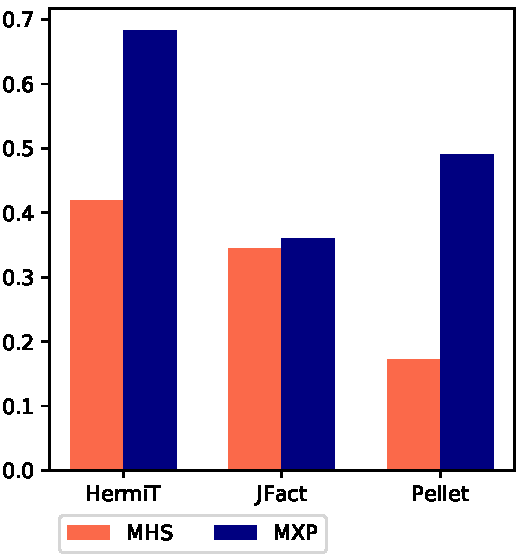
\includegraphics[width=11cm]{eval1Family}
	\caption{Family ontology - Experiment 1}
	\label{fig:eval1Family}
\end{figure}

The second tested ontology was the Beer ontology. The result from the experiment on this ontology we can see in the Figure~\ref{fig:eval1Beer}. The Beer ontology is significantly bigger than the Family ontology. We can see that the JFact reasoner was definitely quicker with the MXP approach. On the other hand the Pellet reasoner was quicker with the MHS algorithm. The HermiT reasoner is also quicker with the MHS algorithm and the implementation of the Hermit reasoner seems to have better performance for larger ontologies. The HermiT reasoner achieved worse results with the Family ontology comparing to the other reasoners and the Family ontology is smaller than the Beer ontology.

\begin{figure}[H]
	\centering
	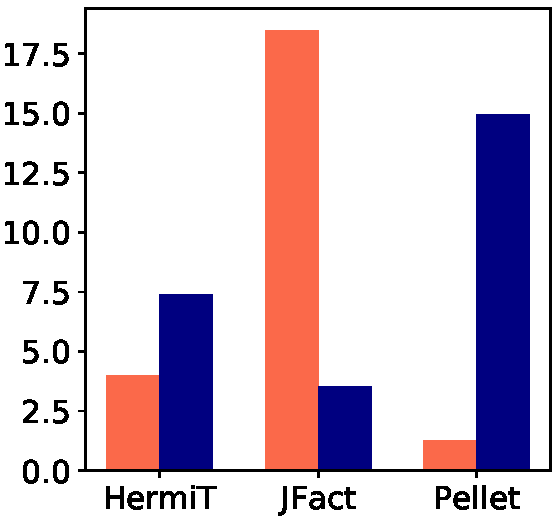
\includegraphics[width=11cm]{eval1Beer} 
	\caption{Beer ontology - Experiment 1}
	\label{fig:eval1Beer}
\end{figure}

The last ontology that has been tested is the LUBM ontology. That is our largest ontology. The result from the experiment on this ontology is in the Figure~\ref{fig:eval1LUBM}. As we can see the JFact reasoner is again extremely slow with the MHS algorithm comparing to MXP algorithm. The Pellet reasoner acts similarly as it did in two previous cases, the MHS algorithm is quicker than the MXP algorithm. The HermiT reasoner is with both approaches in the middle, the MHS algorithm was quicker with the Pellet reasoner, the MXP algorithm was quicker with the JFact reasoner.

\begin{figure}[H]
	\centering
	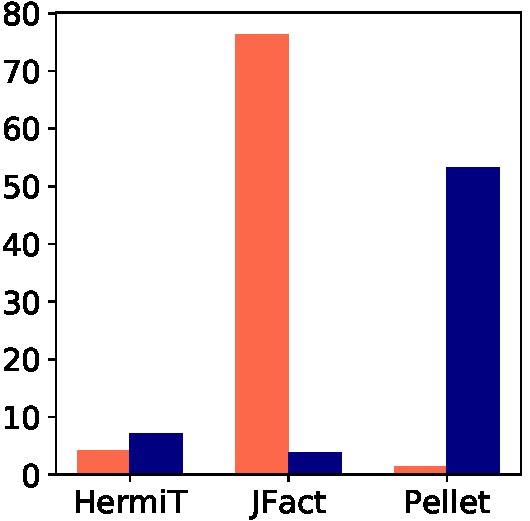
\includegraphics[width=11cm]{eval1LUBM} 
	\caption{LUBM ontology - Experiment 1}
	\label{fig:eval1LUBM}
\end{figure}

\subsection{Experiment 2}
Experiment 2 compares execution times between the MHS and the MXP algorithm. The MHS algorithm was launched with the timeout parameter and the timeout was set to 43200 seconds which is 12 hours. The MXP algorithm finished without any timeout. In this experiment we want to compare execution times and number of found explanations expressed in percentage. We assume that the MHS algorithm will find all possible explanations and we take its count as maximum or in other words as 100\% of all minimal explanations. Then we calculate how much percentage of minimal explantions the MXP algorithm was able to find. In this experiment all resulting plots show the percentage of found minimal explanations at the top of the bar in the histogram. Under each plot the legend is displayed. Each legend describes if the used algorithm is the MHS or the MXP algorithm and in the case of the MHS algorithm the legend shows the depth of the HS-tree. Each depth is displayed with different saturation of the red color. Each observation ends in different depth. Each depth is calculated as an average of 10 runs from 10 observations. Let us say that in the plot we have 5 depths. That means that at least one observation achieved the fifth depth. But it does not mean that each observation finished in the fifth depth. An average of this depth is calculated also as an average of 10 runs from 10 observation but execution time of observations that did not achieve this depth is zero.

\begin{figure}[H]
	\centering
	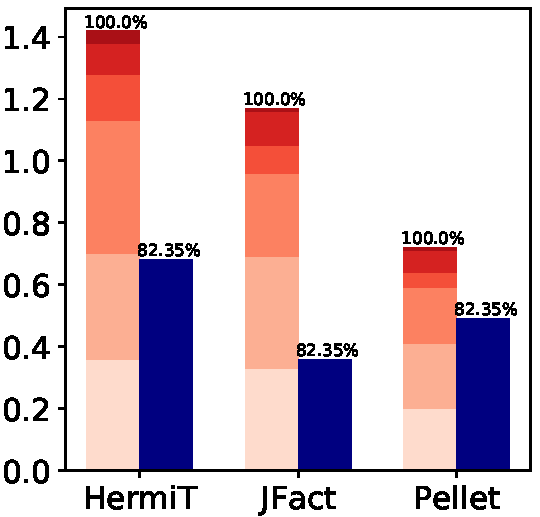
\includegraphics[width=10cm]{eval2Family} 	
	\caption{Family ontology - Experiment 2}
	\label{fig:eval2Family}
\end{figure}

The Family ontology is the first ontology that has been tested in our experiment. The resulting plot we can see in the Figure~\ref{fig:eval2Family}. This ontology is small so both algorithms finished their goal without timeout. With all three reasoners the MXP approach found exactly the same number of minimal explanations because the percentage is the same. This ontology is interesting for its structure. There is a multiple hierarchy in concepts and that is why a simple observation can have minimal explanations with cardinality bigger than one. The MXP algorithm is not able to find all minimal explanations which cardinality is bigger than one. So the resulting percentage is not 100\%. 

This experiment is measured in seconds but in the plot in Figure~\ref{fig:eval2Family} we can see that the MXP algorithm is with any of tested reasoners quicker than the MHS algorithm. The MHS algorithm has found all minimal explanations but it was definitely slower. The HermiT reasoner is the slowest and the Pellet reasoner is the quickest. Interestingly, it cannot be stated that if one reasoner is the quickest with the MHS approach it will be also the quickest with the MXP approach. Great example is the JFact reasoner with the Family ontology. The JFact reasoner is the quickest reasoner with the MXP approach but is the second best reasoner with the MHS approach.

The Beer ontology is used as the second ontology in Experiment 2. We can see its result on Figure~\ref{fig:eval2Beer}. The MXP approach takes only seconds and therefore we cannot see it in the plot in Figure~\ref{fig:eval2Beer}. This plot is displayed in hours because the MHS algorithm took a long time. But the MXP algorithm was running only a few seconds. For the MHS approach a 12 hours timeout has to be set. And we can see that HermiT and JFact have managed to run this 12 hours but Pellet did not. The reason why Pellet took shorter time is not that it was that quick. It is because the Pellet reasoner threw an exception (OutOfMemoryException). That is not problem with our algorithm, that is a problem with the reasoner. The Pellet reasoner checks consistency by doing the Tableau algorithm which is an exponential algorithm. Pellet is probably implemented so that it requires a lot of memory. 

\begin{figure}[H]
	\centering
	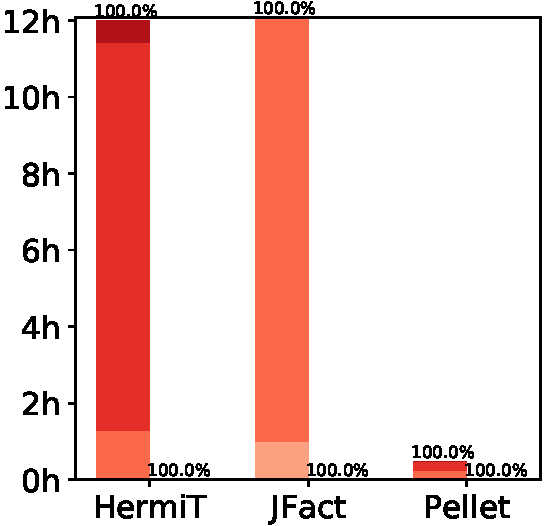
\includegraphics[width=10cm]{eval2Beer} 
	\caption{Beer ontology - Experiment 2}
	\label{fig:eval2Beer}
\end{figure}

We assume that minimal explanations that have been found before timeout are our 100\% of all minimal explanations. And we compare this result with the MXP approach and its result. The Beer ontology is bigger than the Family ontology and it has different structure. The Beer ontology is flat, the maximum depth of a concept hierarchy is two. So that means that we can assume that explanations of simple observation will be probably of size one. The MXP algorithm has to find all minimal explanations in such a case. We have confirmed that the MXP algorithm has found all minimal explanations that were found by the MHS approach. We can observe that each reasoner finished in different depth before timeout. The HermiT reasoner managed to get into the third depth of the HS-tree, the JFact reasoner was only in the second and the Pellet reasoner seems to be the quickest because it was in the second depth before the other reasoners. Unfortunately the Pellet reasoner threw an OutOfMemoryException and could not finish.


The third ontology is the LUBM ontology in our experiment. Its result we can see in Figure~\ref{fig:eval2LUBM}. The LUBM ontology is bigger than the Beer ontology but its structure is similar to the Beer ontology. Also the resulting plot is similar to the plot with the Beer ontology. Again the MXP approach took only seconds and therefore it cannot be seen in the plot. The plot is displayed in hours. The Pellet reasoner threw an OutOfMemoryException so it finished earlier. The HermiT and Pellet reasoner were terminated because of the timeout. Both reasoners did not finish naturally but we assume that they have found 100\% of all explanations. The MXP approach found also 100\% comparing to the MHS algorithm. But the LUBM ontology has similar structure as the Beer ontology. Its structure is flat so we cannot find minimal explanations with cardinality bigger than one.

\begin{figure}[H]
	\centering
	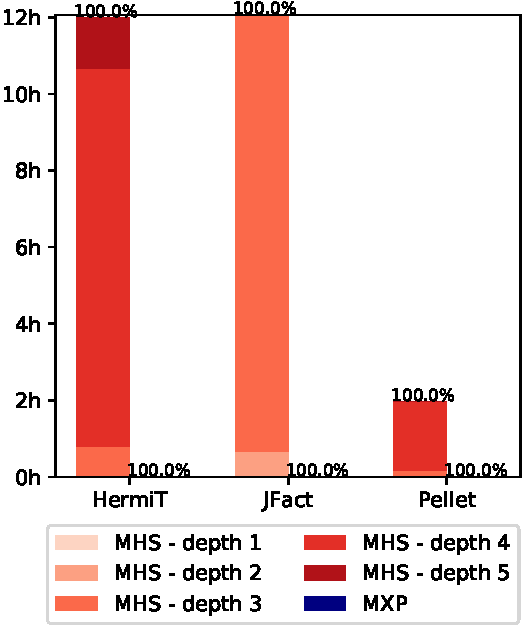
\includegraphics[width=10cm]{eval2LUBM} 
	\caption{LUBM ontology - Experiment 2}
	\label{fig:eval2LUBM}
\end{figure}

\subsection{Conclusion from Experiments}
Experiment 1 finished in all cases without timeout and without any exceptions. In general we can say that the MXP algorithm found all minimal explanations with cardinality equals to one. We know that the MHS algorithm is sound and complete so we assume that all found minimal explanations are really all and no other minimal explanation exists. That is why we say that the MXP algorithm has found all minimal explanations comparing to the MHS algorithm. By comparing result from the MXP and the MHS approach we can see that in this case is more useful to use the MHS algorithm because it is quicker, except JFact reasoner. But that could be due to the implementation of this reasoner. Interesting about JFact is that with the MHS approach is the slowest reasoner. But with the MXP approach it is not the slowest reasoner. So we cannot say that the JFact reasoner is not suitable for our solution.

In Experiment 2 a timeout needed to be set. The timeout was set to 12 hours and for bigger ontologies like the Beer and the LUBM ontology it was still not enough. They did not manage to finish and they were terminated because of the timeout. The Family ontology is a small ontology so it finished before timeout was reached. This ontology finished in seconds in our experiment. This experiment was about to find all possible minimal explanations, not just minimal explanations of size one. The goal of this experiment is to compare what percentage of all possible minimal explanations could be found by the MXP algorithm. The experiment did not find 100\% of minimal explanations only with the Family ontology. That is because its structure is more hierarchical comparing to the other two ontologies. The experiment found all minimal explanations with these two ontologies. The execution times with both approaches are very different. With the Family ontology we can see that there is no such big difference, it is just a few seconds because the ontology is small. But with the Beer and the LUBM ontology we can see that the MHS algorithm took hours and it still was not enough and the MXP algorithm took only seconds and it found all minimal explanations.

We assume that the MXP algorithm can find all minimal explanations of size one. We can see it in both experiments where this algorithm has found all minimal explanations of size one. It is more suitable for ontologies with flat hierarchy. But that depends on the situation. If we prefer to find only minimal explanations with the cardinality equals to one, then we can definitely use the MXP approach. Or if we have ontologies like the Beer or the LUBM ontology that are big but flat then we can also use the MXP algorithm to find minimal explanations. But with this situation we can also use the MHS approach with defined depth parameter.

\pagebreak
\section{Conclusions}
We wanted to find out if the MergeXPlain algorithm is the solution for the ABox abduction problem. From evaluation part we assume that the MXP algorithm will find all minimal explanations of size one. But we cannot guarantee that the MXP will find all minimal explanations. So the answer for our question is not so simple. We cannot say that the MHS algorithm takes too long and can be replaced with the MXP algorithm. We can say that for some situations where we have ontologies with flat hierarchy we can use the MXP algorithm or we can use the MHS algorithm with depth parameter set to one.

The goal of our thesis was to implement two approaches and compare their execution times and results. We managed to implement both approaches to work correctly. In the process of implementation we have found out that the MXP algorithm is not able to find all minimal explanations. This happens if there are some minimal explanations which are overlapping with each other. Then the MXP algorithm will not find them all, it will find only a subset of them. That is happening because the MXP algorithm is not able to search the whole space of possible explanations. But if we have minimal explanations that do not overlap with each other, the MXP algorithm should find them. The evaluation showed that the MXP algorithm can be used if we look only for minimal explanations of size one. Experiment 1 showed that if we look only for minimal explanations with cardinality equals to one we want to use the MHS algorithm because it is a little bit quicker. Experiment 2 showed in the case with the Family ontology that even if the MXP will not find all explanations, it found 83\% which is not so bad. 

An interesting question for future work is if both approaches can be combined. The advantage of the MXP algorithm is its speed. The slow part of the MHS algorithm is to compute the negated model for given node. This step could be replaced with the MXP algorithm and that could improve the execution times.

\pagebreak
\bibliography{references}
\bibliographystyle{unsrtnat}

\end{document}